\documentclass[]{report}
\usepackage{lmodern}
\usepackage{amssymb,amsmath}
\usepackage{ifxetex,ifluatex}
\usepackage{fixltx2e} % provides \textsubscript
\ifnum 0\ifxetex 1\fi\ifluatex 1\fi=0 % if pdftex
  \usepackage[T1]{fontenc}
  \usepackage[utf8]{inputenc}
\else % if luatex or xelatex
  \ifxetex
    \usepackage{mathspec}
  \else
    \usepackage{fontspec}
  \fi
  \defaultfontfeatures{Ligatures=TeX,Scale=MatchLowercase}
\fi
% use upquote if available, for straight quotes in verbatim environments
\IfFileExists{upquote.sty}{\usepackage{upquote}}{}
% use microtype if available
\IfFileExists{microtype.sty}{%
\usepackage{microtype}
\UseMicrotypeSet[protrusion]{basicmath} % disable protrusion for tt fonts
}{}
\usepackage[margin=1in]{geometry}
\usepackage{hyperref}
\hypersetup{unicode=true,
            pdfauthor={Samuel Lippl},
            pdfborder={0 0 0},
            breaklinks=true}
\urlstyle{same}  % don't use monospace font for urls
\usepackage{natbib}
\bibliographystyle{apalike}
\usepackage{color}
\usepackage{fancyvrb}
\newcommand{\VerbBar}{|}
\newcommand{\VERB}{\Verb[commandchars=\\\{\}]}
\DefineVerbatimEnvironment{Highlighting}{Verbatim}{commandchars=\\\{\}}
% Add ',fontsize=\small' for more characters per line
\usepackage{framed}
\definecolor{shadecolor}{RGB}{248,248,248}
\newenvironment{Shaded}{\begin{snugshade}}{\end{snugshade}}
\newcommand{\KeywordTok}[1]{\textcolor[rgb]{0.13,0.29,0.53}{\textbf{#1}}}
\newcommand{\DataTypeTok}[1]{\textcolor[rgb]{0.13,0.29,0.53}{#1}}
\newcommand{\DecValTok}[1]{\textcolor[rgb]{0.00,0.00,0.81}{#1}}
\newcommand{\BaseNTok}[1]{\textcolor[rgb]{0.00,0.00,0.81}{#1}}
\newcommand{\FloatTok}[1]{\textcolor[rgb]{0.00,0.00,0.81}{#1}}
\newcommand{\ConstantTok}[1]{\textcolor[rgb]{0.00,0.00,0.00}{#1}}
\newcommand{\CharTok}[1]{\textcolor[rgb]{0.31,0.60,0.02}{#1}}
\newcommand{\SpecialCharTok}[1]{\textcolor[rgb]{0.00,0.00,0.00}{#1}}
\newcommand{\StringTok}[1]{\textcolor[rgb]{0.31,0.60,0.02}{#1}}
\newcommand{\VerbatimStringTok}[1]{\textcolor[rgb]{0.31,0.60,0.02}{#1}}
\newcommand{\SpecialStringTok}[1]{\textcolor[rgb]{0.31,0.60,0.02}{#1}}
\newcommand{\ImportTok}[1]{#1}
\newcommand{\CommentTok}[1]{\textcolor[rgb]{0.56,0.35,0.01}{\textit{#1}}}
\newcommand{\DocumentationTok}[1]{\textcolor[rgb]{0.56,0.35,0.01}{\textbf{\textit{#1}}}}
\newcommand{\AnnotationTok}[1]{\textcolor[rgb]{0.56,0.35,0.01}{\textbf{\textit{#1}}}}
\newcommand{\CommentVarTok}[1]{\textcolor[rgb]{0.56,0.35,0.01}{\textbf{\textit{#1}}}}
\newcommand{\OtherTok}[1]{\textcolor[rgb]{0.56,0.35,0.01}{#1}}
\newcommand{\FunctionTok}[1]{\textcolor[rgb]{0.00,0.00,0.00}{#1}}
\newcommand{\VariableTok}[1]{\textcolor[rgb]{0.00,0.00,0.00}{#1}}
\newcommand{\ControlFlowTok}[1]{\textcolor[rgb]{0.13,0.29,0.53}{\textbf{#1}}}
\newcommand{\OperatorTok}[1]{\textcolor[rgb]{0.81,0.36,0.00}{\textbf{#1}}}
\newcommand{\BuiltInTok}[1]{#1}
\newcommand{\ExtensionTok}[1]{#1}
\newcommand{\PreprocessorTok}[1]{\textcolor[rgb]{0.56,0.35,0.01}{\textit{#1}}}
\newcommand{\AttributeTok}[1]{\textcolor[rgb]{0.77,0.63,0.00}{#1}}
\newcommand{\RegionMarkerTok}[1]{#1}
\newcommand{\InformationTok}[1]{\textcolor[rgb]{0.56,0.35,0.01}{\textbf{\textit{#1}}}}
\newcommand{\WarningTok}[1]{\textcolor[rgb]{0.56,0.35,0.01}{\textbf{\textit{#1}}}}
\newcommand{\AlertTok}[1]{\textcolor[rgb]{0.94,0.16,0.16}{#1}}
\newcommand{\ErrorTok}[1]{\textcolor[rgb]{0.64,0.00,0.00}{\textbf{#1}}}
\newcommand{\NormalTok}[1]{#1}
\usepackage{longtable,booktabs}
\usepackage{graphicx,grffile}
\makeatletter
\def\maxwidth{\ifdim\Gin@nat@width>\linewidth\linewidth\else\Gin@nat@width\fi}
\def\maxheight{\ifdim\Gin@nat@height>\textheight\textheight\else\Gin@nat@height\fi}
\makeatother
% Scale images if necessary, so that they will not overflow the page
% margins by default, and it is still possible to overwrite the defaults
% using explicit options in \includegraphics[width, height, ...]{}
\setkeys{Gin}{width=\maxwidth,height=\maxheight,keepaspectratio}
\IfFileExists{parskip.sty}{%
\usepackage{parskip}
}{% else
\setlength{\parindent}{0pt}
\setlength{\parskip}{6pt plus 2pt minus 1pt}
}
\setlength{\emergencystretch}{3em}  % prevent overfull lines
\providecommand{\tightlist}{%
  \setlength{\itemsep}{0pt}\setlength{\parskip}{0pt}}
\setcounter{secnumdepth}{5}

%%% Use protect on footnotes to avoid problems with footnotes in titles
\let\rmarkdownfootnote\footnote%
\def\footnote{\protect\rmarkdownfootnote}

%%% Change title format to be more compact
\usepackage{titling}

% Create subtitle command for use in maketitle
\newcommand{\subtitle}[1]{
  \posttitle{
    \begin{center}\large#1\end{center}
    }
}

\setlength{\droptitle}{-2em}

  \title{}
    \pretitle{\vspace{\droptitle}}
  \posttitle{}
    \author{Samuel Lippl}
    \preauthor{\centering\large\emph}
  \postauthor{\par}
      \predate{\centering\large\emph}
  \postdate{\par}
    \date{2018-09-15}

\usepackage{booktabs, titlesec, blindtext}
\usepackage[svgnames]{xcolor}
\hypersetup{
    bookmarksnumbered=true,
    bookmarksopen=false,
    bookmarksopenlevel=1,
    colorlinks=true,
    linkcolor=blue,
    urlcolor=DarkBlue,
    citecolor=DarkRed
}
\definecolor{chgray}{gray}{0.5}
\newcommand{\hsp}{\hspace{20pt}}
\titleformat{\chapter}[hang]{\Huge\bfseries}{\thechapter\hsp\textcolor{chgray}{|}\hsp}{0pt}{\Huge\bfseries}

\usepackage{amsthm}
\newtheorem{theorem}{Theorem}[chapter]
\newtheorem{lemma}{Lemma}[chapter]
\theoremstyle{definition}
\newtheorem{definition}{Definition}[chapter]
\newtheorem{corollary}{Corollary}[chapter]
\newtheorem{proposition}{Proposition}[chapter]
\theoremstyle{definition}
\newtheorem{example}{Example}[chapter]
\theoremstyle{definition}
\newtheorem{exercise}{Exercise}[chapter]
\theoremstyle{remark}
\newtheorem*{remark}{Remark}
\newtheorem*{solution}{Solution}
\begin{document}

\begin{titlepage}

% Titlepage inspired by: https://www.overleaf.com/15991102jmmvbxxtbhfk#/61015645/

\newcommand{\HRule}{\rule{\linewidth}{0.5mm}} % Defines a new command for the horizontal lines, change thickness here

\center % Center everything on the page

%----------------------------------------------------------------------------------------
%	TITLE SECTION
%----------------------------------------------------------------------------------------

\HRule \\[0.4cm]
{ \huge \bfseries Description, implementation and validation of a user interface for complex datasets in the social sciences}\\[0.4cm] % Title of your document
\HRule \\[1.5cm]

%----------------------------------------------------------------------------------------
%	HEADING SECTIONS
%----------------------------------------------------------------------------------------

\textsc{\LARGE Ludwig-Maximilians-Universität München}\\[0.5cm] % Name of your university/college
\textsc{\Large Fakultät für Mathematik, Informatik und Statistik}\\[1.5cm]


\textsc{\Large Bachelor of Statistics}\\[0.5cm] % Major heading such as course name
\textsc{\large Bachelor's Thesis}\\[0.5cm] % Minor heading such as course title

%----------------------------------------------------------------------------------------
%	LOGO SECTION
%----------------------------------------------------------------------------------------

\vfill


\includegraphics[height=0.2\textheight]{figs/sigill.png}\\[1cm] % Include a department/university logo - this will require the graphicx package



%----------------------------------------------------------------------------------------
%	DATE SECTION
%----------------------------------------------------------------------------------------

\vfill

%----------------------------------------------------------------------------------------
%	AUTHOR SECTION
%----------------------------------------------------------------------------------------

{\Large 30. Juni 2018}\\[1cm]
\begin{Large}
\textsc{Author}\\Samuel Lippl\\[1cm]
\textsc{Supervisor}\\
Dr. Fabian Scheipl
\end{Large}

\vfill

\end{titlepage}

\pagenumbering{roman}
\setcounter{page}{2}

\chapter*{Selbständigkeitserklärung}

Ich erkläre hiermit, dass ich die vorliegende Arbeit selbständig angefertigt, alle Zitate als solche kenntlich gemacht sowie alle benutzten Quellen und Hilfsmittel angegeben habe.\\

\begin{tabular}{c}
\\\\\\
\\\hline
Samuel Lippl, 15.09.2018
\end{tabular}

\chapter*{Abstract}\label{abstract}


This report will provide an overview over outlier detection in R. It
starts by discussing some general principles of outlier detection.
Linear methods and their nonlinear extensions are presented next. Along
the general methods, examples of application and an appropriate
methodology in R are introduced. The report will be concluded by a
discussion of method evaluation as well as a comparison of the different
introduced algorithms.

\tableofcontents

\chapter{Introduction}\label{intro}

\pagenumbering{arabic} \setcounter{page}{1}

One of the main advantages of the statistical programming language R
\citep{R} lies in its conciseness. With just one line of code, it is
possible to build a linear model, visualize a variable's distribution or
conduct complex modifications on several datasets. This is possible
because R is a domain-specific language and is therefore able to make
strong assumptions -- many people will need to build a linear model or
read in a csv file and it is therefore sensible to create custom
functions for these purpose.

An important property of this conciseness is that the code is still easy
to read. Two features that are especially important for this both rely
on the specific domain of statistical analysis for which R was created:

\begin{itemize}
\item
  \emph{Specialized functions:} \texttt{read.csv} essentially calls
  \texttt{read.table} with a few modified parameters. Nonetheless, the
  function immediately makes it clear what this line of code is supposed
  to achieve.
\item
  \emph{Default values:} The user does not need to specify every single
  parameter of a function. For instance, it is helpful that
  \texttt{read.table} contains the parameter \texttt{na.strings} that
  allows the user to specify values that encode \texttt{NA}s. However,
  in most cases, \texttt{NA}s are encoded by the string \texttt{NA} or a
  missing value \footnote{The latter is only implemented in
    \texttt{read\_delim} from the package \texttt{readr} but the
    advantage of default values remains valid nevertheless.}. By setting
  default values, the user only needs to think about this parameter when
  the file structure is out of the ordinary.
\end{itemize}

These advantages are certainly not unique to R. They are designed to
minimize the expected time a user needs to spend with coding his
decisions while maintaining easy reproducibility of his work. On the
other hand, if there are more complicated tasks to undertake, a
consistent interface allows the user to do that, as well.

A good example for this concept, in my mind, is the package
\texttt{stringr} \citep{stringr}. Functions like \texttt{str\_trim}
(trim whitespace) or \texttt{str\_to\_title} (capitalize) make special
use cases easily accessible. On the other hand, \texttt{str\_replace}
allows more complicated operations with regular expressions using the
same consistent interface.

Things, however, start to fall apart when one attempts to modify default
values. This is sometimes possible by setting the global options in R;
however, relying on these makes reproducibility harder. On the other
hand, one could write new functions to solve this problem. This is,
however, more laborious than such an endeavour needs to be.

A good example of this are datasets with many variables as they occur in
the social sciences. As an example, I will consider the Varieties of
Democracy (\href{v-dem.net}{V-Dem}) dataset which produces indicators of
democracy \citep[\citet{Pemstein2018}]{vdem2018}. It contains many
variables on different aspects of democracy with values per country and
year. If one wishes to visualize the development of this variable over
time, a simple line plot often makes sense. Consider, for instance, the
variable which characterizes the freedom of religion on a scale between
0 and 4 for Germany in figure \ref{fig:ex1}.

\begin{figure}

{\centering 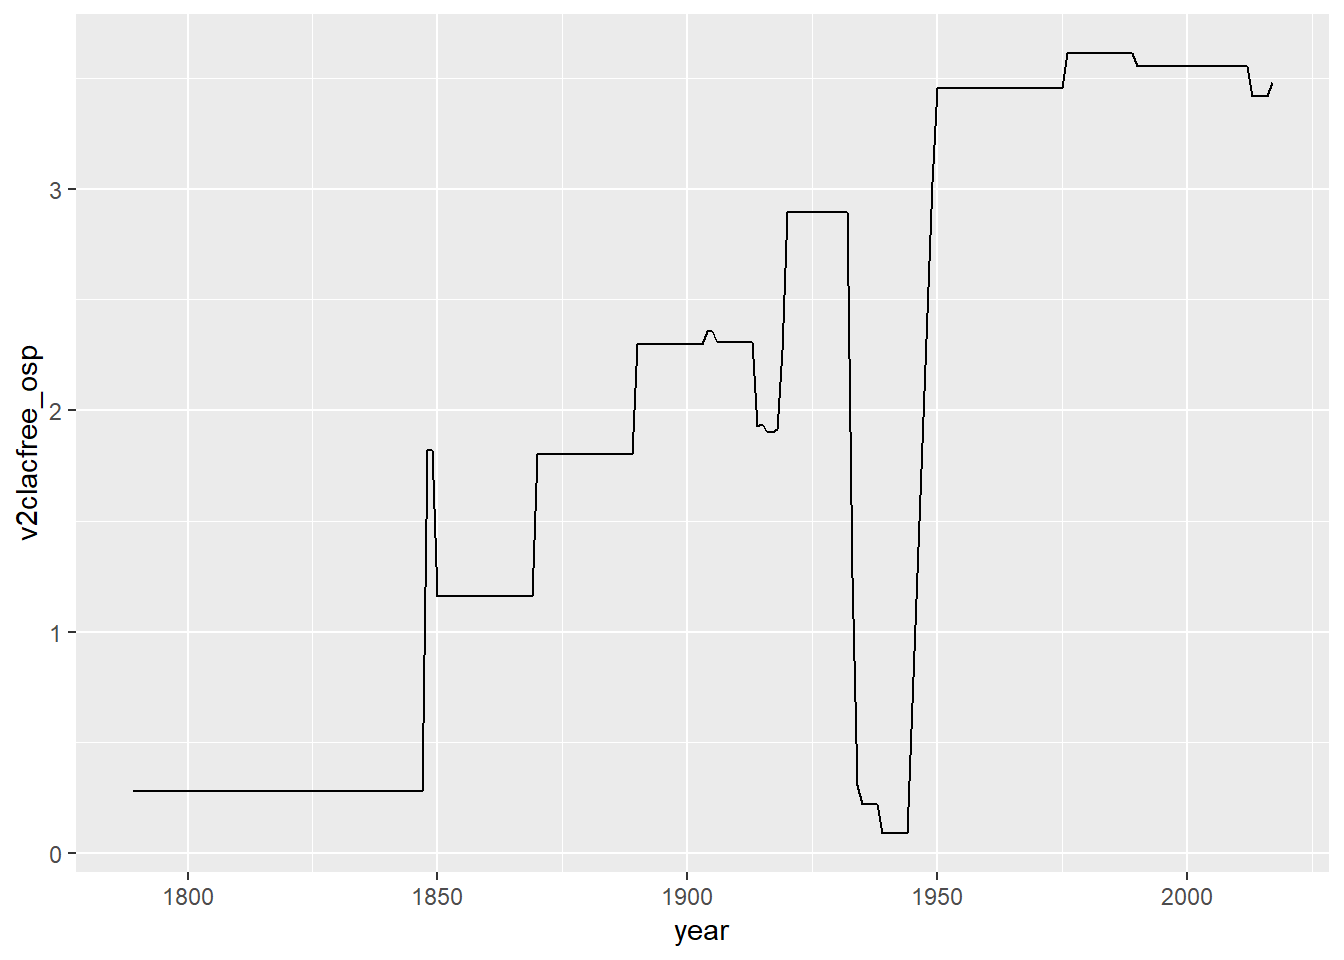
\includegraphics[width=0.5\linewidth]{bachelor-thesis_files/figure-latex/ex1-1} 

}

\caption{Example: Freedom of religion in Germany over time}\label{fig:ex1}
\end{figure}

Although there are considerable changes within a single year, freedom of
religion is a continuous value and linear interpolation of this
development within a year makes sense.

Considering the variable \texttt{v2elvotbuy\_osp}, however, a line plot
makes less sense. This variable captures whether there was evidence of
vote buying during a national election and is therefore only present in
years where there has been a national election. A step plot as depicted
in figure \ref{fig:ex2} seems more sensible in this case as the current
value would always refer to the last election.

\begin{figure}

{\centering 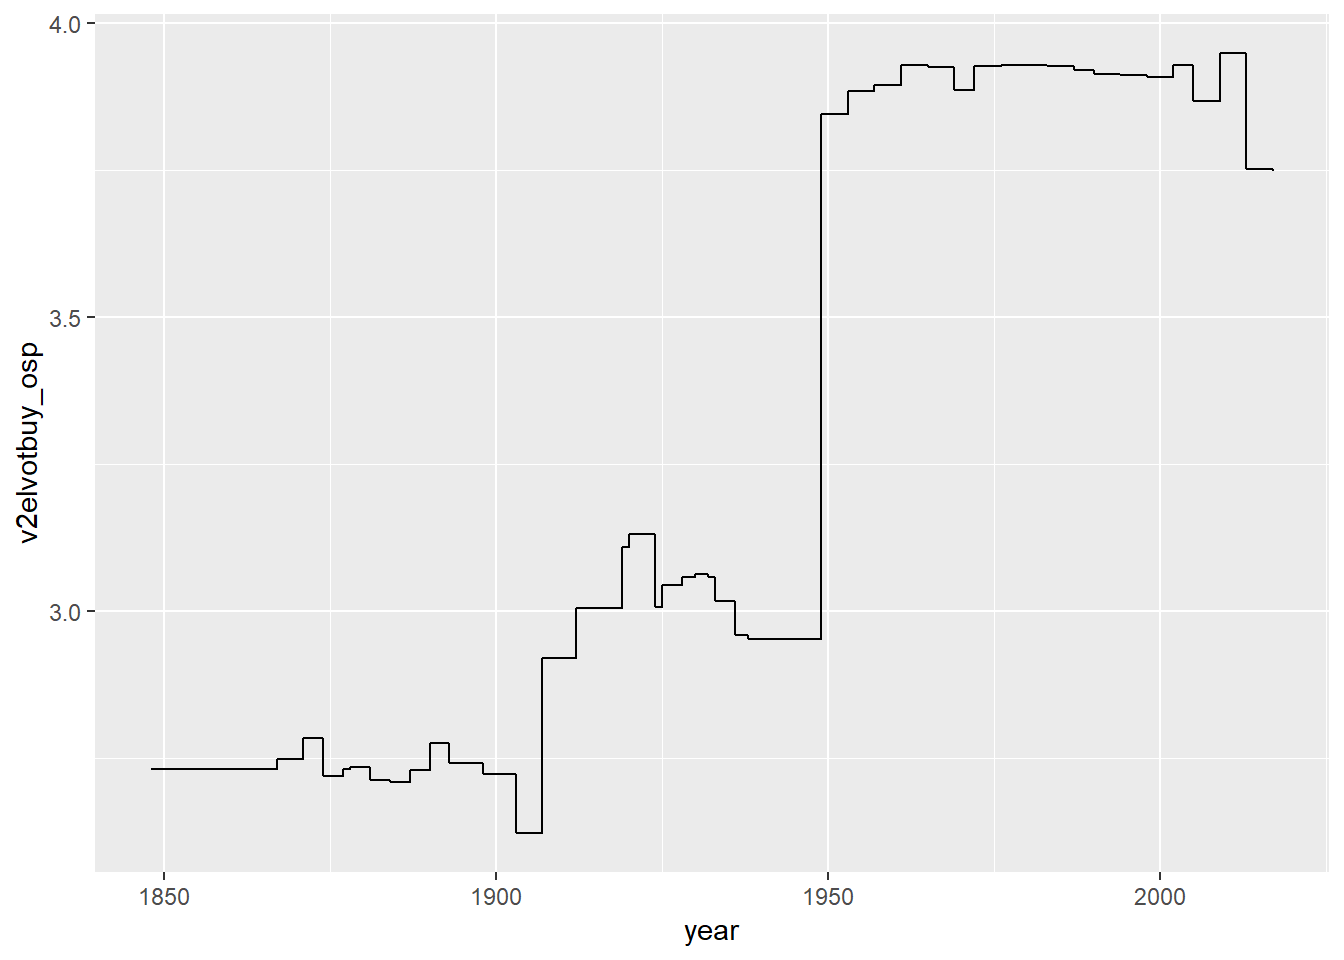
\includegraphics[width=0.5\linewidth]{bachelor-thesis_files/figure-latex/ex2-1} 

}

\caption{Example: Election vote buying in Germany over time}\label{fig:ex2}
\end{figure}

Furthermore, the scale titles should be modified to show an
interpretable variable name, the scale should in most cases be
standardized to depict the entire range between 0 and 4.

In summary, there are many considerations one needs to regard in such a
visualization. Therefore, every time the statistician needs to implement
such a visualization, she needs to think about these questions again,
which is time expensive and makes interactive user interfaces
impossible. This problem is not limited to visualization; another
example would be descriptive tables of a linear model or a report
summarizing all covariates that have been used.

In summary, R provides amazing opportunities to outsource everyday
thought processes in data analysis. However, adapting these mechanisms
for application-specific thought processes is expensive and difficult. A
broad framework for such an adaptation would enable researchers to think
about certain decisions (like the visualization of a specific variable)
once and then be done with it. Both the researcher himself and his
colleagues who might not need to think about this at all would benefit
from this.

In this Bachelor's Thesis, I describe such a framework, implement it as
the package \texttt{tectr} in R and apply it to the V-DEM dataset. The
\protect\hyperlink{methods}{next chapter} discusses some details
regarding the package construction and the dataset before we get a
\protect\hyperlink{example}{first look} in the third chapter. The
\protect\hyperlink{concept}{fourth chapter} will present the framework
and the implementation in a more specific way.
\protect\hyperlink{application}{Chapter five} presents the application
of \texttt{tectr} to the V-DEM dataset and the
\protect\hyperlink{summary}{final chapter} summarizes the thesis and
discusses the next steps regarding \texttt{tectr}.

\hypertarget{methods}{\chapter{Methodology}\label{methods}}

This chapter introduces the V-Dem dataset and discuss the methodological
background of \texttt{tectr}'s construction.

\section{V-Dem}\label{v-dem}

\subsection{Introduction to the
database}\label{introduction-to-the-database}

The Varieties of Democracy Institute is concerned with measuring
different aspects of democracy. It distinguishes between seven
high-level principles: electoral, liberal, participatory, deliberative,
egalitarian, majoritarian and consensual. These are measured by a
variable in the interval \([0,1]\) and each consists of several mid- and
low-level indices. The low-level indices are coded with the help of
several country experts who answer a detailed questionnaire. Most
questions can be answered by an ordinal scale of five alternatives.
Consider, as an example, the variable ``Disclosure of campaign
donations'':

\begin{quote}
\textbf{Are there disclosure requirements for donations to national
election campaigns?}

0: No. There are no disclosure requirements.

1: Not really. There are some, possibly partial, disclosure requirements
in place but they are not observed or enforced most of the time.

2: Ambiguous. There are disclosure requirements in place, but it is
unclear to what extent they are observed or enforced.

3: Mostly. The disclosure requirements may not be fully comprehensive
(some donations not covered), but most existing arrangements are
observed and enforced.

4: Yes. There are comprehensive requirements and they are observed and
enforced almost all the time.
\end{quote}

The answers are then analyzed for inter-coder reliability and a
standardized average of the responses together with a confidence
interval which contains 68 \% of the probability mass is created.
Lower-level indices are created from these answers which are summarized
in mid-level and then high-level indices. An overview over the structure
can be found in appendix D of the codebook \citep{vdem-codebook2018}.
The database contains data on 201 countries between 1789 and 2017.
\citep[\citet{Pemstein2018}]{vdem2018}

\subsection{\texorpdfstring{\texttt{vdem.tectr}}{vdem.tectr}}\label{vdem.tectr}

I have created the package \texttt{vdem.tectr} which contains the
country-year dataset version 8. It can be downloaded via
\href{github.com/sflippl/vdem.tectr}{github}:

\begin{Shaded}
\begin{Highlighting}[]
\CommentTok{# install.packages("devtools")}
\NormalTok{devtools}\OperatorTok{::}\KeywordTok{install_github}\NormalTok{(}\StringTok{"sflippl/vdem.tectr"}\NormalTok{)}
\end{Highlighting}
\end{Shaded}

The package contains three datasets:

\begin{itemize}
\tightlist
\item
  \texttt{df\_vdem}: This dataset contains all variables from the
  varieties of democracy dataset where interval variables are numeric
  and categorical variables are saved as factors or ordered factors
  where appropriate.
\item
  \texttt{vdem\_spatial}: This \emph{simple features} object \citep{sf}
  contains the polygon shapes of the different countries for every year
  between 1945 and 2017. The borders in 2017 can be seen in
  \ref{fig:vdem-spatial}. I have used the CShapes dataset
  \citep[\citet{Weidmann2010a}]{Weidmann2010}, sovereignty- and
  state-level maps data from \href{www.naturalearthdata.com}{Natural
  Earth} and the details from the document on country coding units from
  V-Dem \citep{Coppedge2018}. Note that the coded country borders by
  V-Dem do not constitute an endorsement of controversial entities such
  as Zanzibar. The function \texttt{vdem\_geocode} makes it possible to
  join the shapes polygons to a data frame as long as the columns
  \texttt{country\_name} and \texttt{year} exist.
\end{itemize}

\begin{figure}
\centering
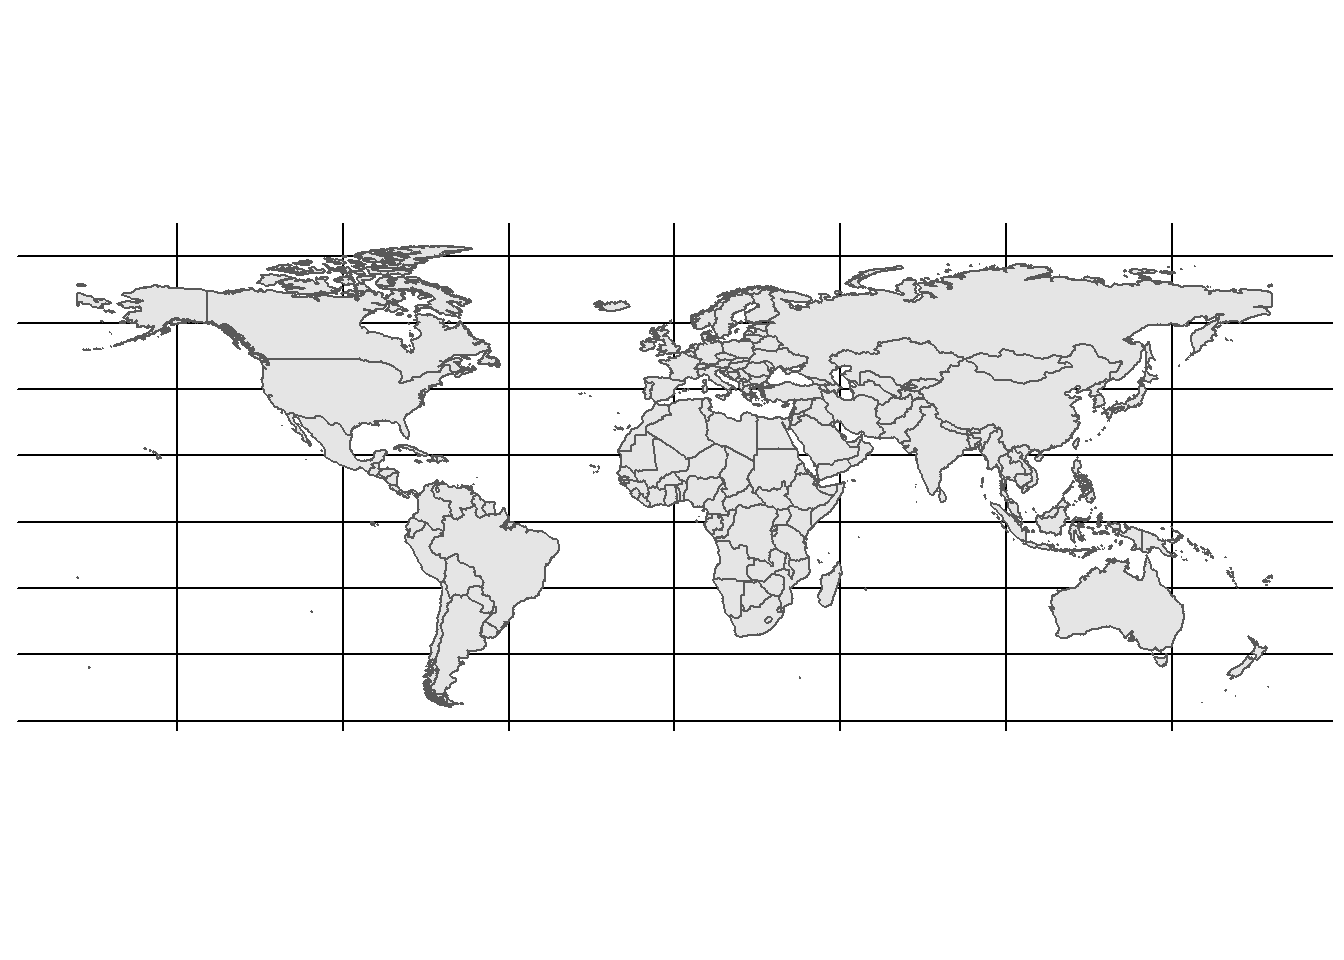
\includegraphics{bachelor-thesis_files/figure-latex/vdem-spatial-1.pdf}
\caption{\label{fig:vdem-spatial}Country borders in 2017 in the V-Dem
database}
\end{figure}

\begin{itemize}
\tightlist
\item
  \texttt{vdem} which contains the variables from \texttt{df\_vdem}, the
  country shapes from \texttt{vdem\_spatial} and further metainformation
  (see \protect\hyperlink{application}{below})
\end{itemize}

Details on these datasets and the reproducible code can be found in the
folder ``data-raw'' in the package.

\section{Package construction}\label{package-construction}

The package has been constructed with the packages \texttt{devtools}
\citep{devtools}, \texttt{roxygen2} \citep{roxygen2} and
\texttt{testthat} \citep{testthat}. The Bachelor's Thesis has been
written with \texttt{bookdown} \citep[\citet{bookdown-2}]{bookdown-1}.

\chapter{First look}\label{first-look}

This chapter is devoted to first applied example of the package before
the \href{fourth\%20chapter}{\#concept} introduces the concepts of
\texttt{tectr} in a more comprehensive way.

As an example, we will consider the V-Dem database that has been
introduced in the preceding chapter. We will focus on the function
\texttt{fx\_ggplot} as an example. It is based on the package
\texttt{ggplot2} which implements the grammar of graphics to R in order
to produce visualizations. \citep{ggplot}

\section{\texorpdfstring{\texttt{fx\_ggplot}:
Basics}{fx\_ggplot: Basics}}\label{fx_ggplot-basics}

We will at first consider the electoral democracy index and its
distribution:

\begin{Shaded}
\begin{Highlighting}[]
\NormalTok{df_vdem }\OperatorTok\StringTok{ }
\StringTok{  }\KeywordTok{select}\NormalTok{(v2x_polyarchy) }\OperatorTok\StringTok{ }
\StringTok{  }\KeywordTok{fx_ggplot}\NormalTok{(}\KeywordTok{aes}\NormalTok{(}\DataTypeTok{x =}\NormalTok{ v2x_polyarchy))}
\end{Highlighting}
\end{Shaded}

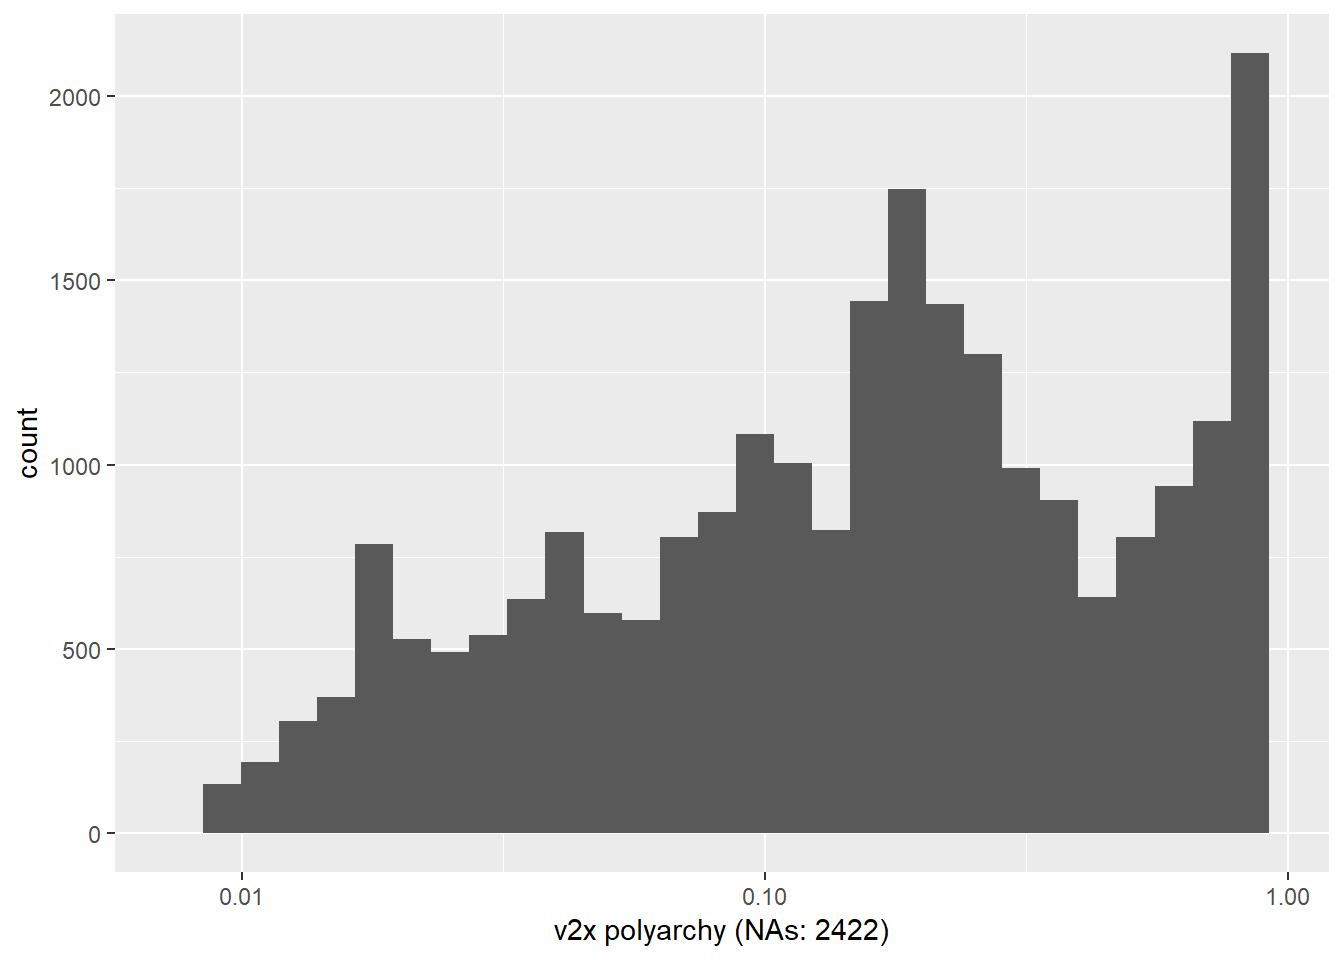
\includegraphics{bachelor-thesis_files/figure-latex/unnamed-chunk-2-1.pdf}

This plot is evidently a histogram. However there are several
differences to the ordinary call:

\begin{Shaded}
\begin{Highlighting}[]
\KeywordTok{ggplot}\NormalTok{(df_vdem, }\KeywordTok{aes}\NormalTok{(}\DataTypeTok{x =}\NormalTok{ v2x_polyarchy)) }\OperatorTok{+}\StringTok{ }\KeywordTok{geom_histogram}\NormalTok{()}
\end{Highlighting}
\end{Shaded}

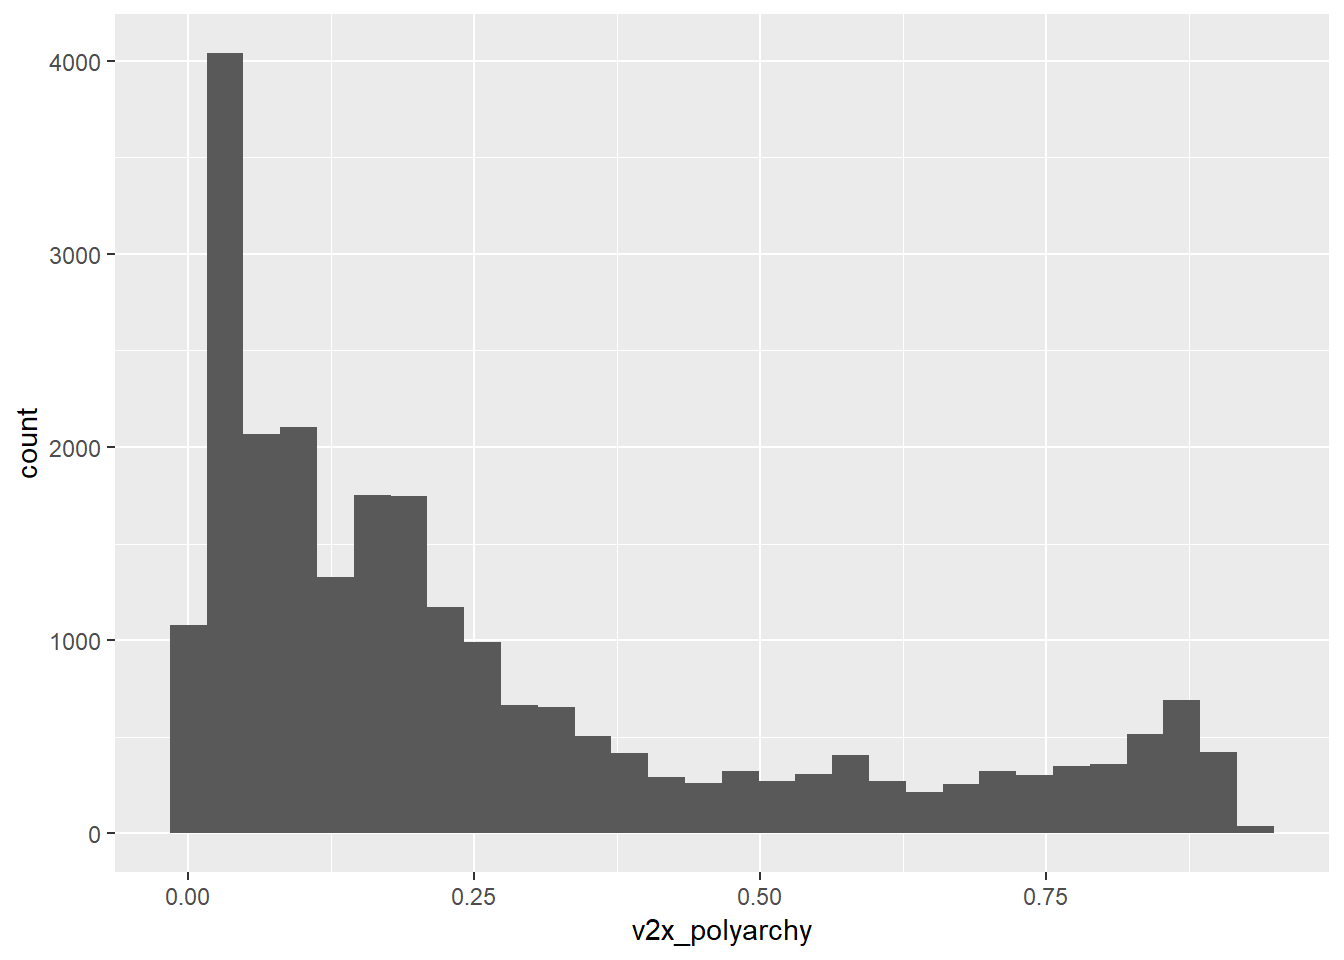
\includegraphics{bachelor-thesis_files/figure-latex/unnamed-chunk-3-1.pdf}

Namely, the axis title lists the number of NAs and the x-axis has been
log transformed. This is because \texttt{tectr} attempts to guess
reasonable default values which yield more informative plots than the
default values of \texttt{ggplot}. It is able to do so because these
default values can flexibly be changed.

Behind the scenes, the function calls \texttt{fx\_default} which sets
several default values for every column and saves them in a
\emph{metaframe} which is stored as an attribute of the data frame.

\begin{Shaded}
\begin{Highlighting}[]
\NormalTok{fx_ggplot_columns}
\end{Highlighting}
\end{Shaded}

\begin{verbatim}
## [1] "fxGeom_class"  "fxGeom_limits" "fxGeom_trans"  "fxInfo_name"
\end{verbatim}

\begin{Shaded}
\begin{Highlighting}[]
\NormalTok{data <-}\StringTok{ }
\StringTok{  }\NormalTok{df_vdem }\OperatorTok\StringTok{ }
\StringTok{  }\KeywordTok{select}\NormalTok{(v2x_polyarchy) }\OperatorTok\StringTok{ }
\StringTok{  }\KeywordTok{fx_default}\NormalTok{(}\DataTypeTok{columns =}\NormalTok{ fx_ggplot_columns)}
\KeywordTok{metaframe}\NormalTok{(data) }\OperatorTok\StringTok{ }
\StringTok{  }\KeywordTok{kable}\NormalTok{(}\DataTypeTok{digits =} \DecValTok{3}\NormalTok{)}
\end{Highlighting}
\end{Shaded}

name

fxGeom\_class

fxGeom\_limits

fxGeom\_trans

fxInfo\_name

v2x\_polyarchy

Continuous

c(0.00728491658127784, 0.939980764975532)

log10

v2x polyarchy

In `fxGeom\_class´, for instance, the class of the variable is listed
which has an influence on the defined graphics and is used to influence
a lot of other default values.

\texttt{fx\_ggplot} itself attempts to infer the appropriate
visualization from the specification of aesthetics and the class of the
data. Thus, we receive a different plot if we specify the y variable, as
well. Let us first consider the relationship between the electoral and
the liberal democracy index in the 2017:

\begin{Shaded}
\begin{Highlighting}[]
\NormalTok{df_vdem }\OperatorTok\StringTok{ }
\StringTok{  }\KeywordTok{filter}\NormalTok{(year }\OperatorTok{==}\StringTok{ }\DecValTok{2017}\NormalTok{) }\OperatorTok\StringTok{ }
\StringTok{  }\KeywordTok{select}\NormalTok{(v2x_polyarchy, v2x_libdem) }\OperatorTok\StringTok{ }
\StringTok{  }\KeywordTok{fx_ggplot}\NormalTok{(}\KeywordTok{aes}\NormalTok{(}\DataTypeTok{x =}\NormalTok{ v2x_polyarchy, }\DataTypeTok{y =}\NormalTok{ v2x_libdem))}
\end{Highlighting}
\end{Shaded}

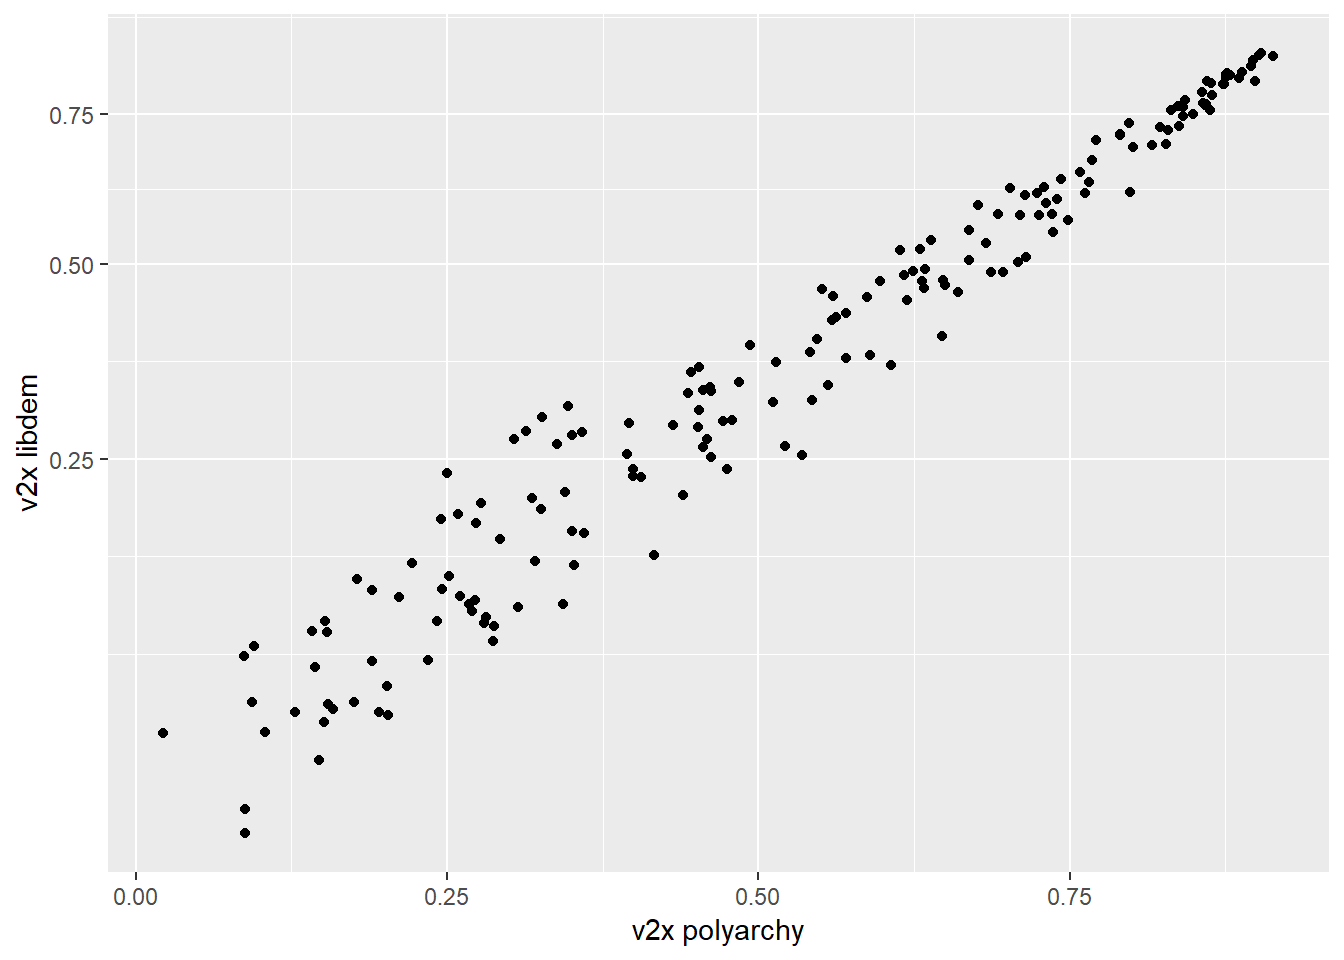
\includegraphics{bachelor-thesis_files/figure-latex/unnamed-chunk-5-1.pdf}

In this case, the scatter plot is a sensible choice. On the other hand,
if we wish to visualize the entire database (which consists of 26537
observations), an ordinary scatter plot would lead to severe
overplotting. \texttt{fx\_ggplot} recognizes this and chooses a more
appropriate graphic:

\begin{Shaded}
\begin{Highlighting}[]
\NormalTok{df_vdem }\OperatorTok\StringTok{ }
\StringTok{  }\KeywordTok{select}\NormalTok{(v2x_polyarchy, v2x_libdem) }\OperatorTok\StringTok{ }
\StringTok{  }\KeywordTok{fx_ggplot}\NormalTok{(}\KeywordTok{aes}\NormalTok{(}\DataTypeTok{x =}\NormalTok{ v2x_polyarchy, }\DataTypeTok{y =}\NormalTok{ v2x_libdem))}
\end{Highlighting}
\end{Shaded}

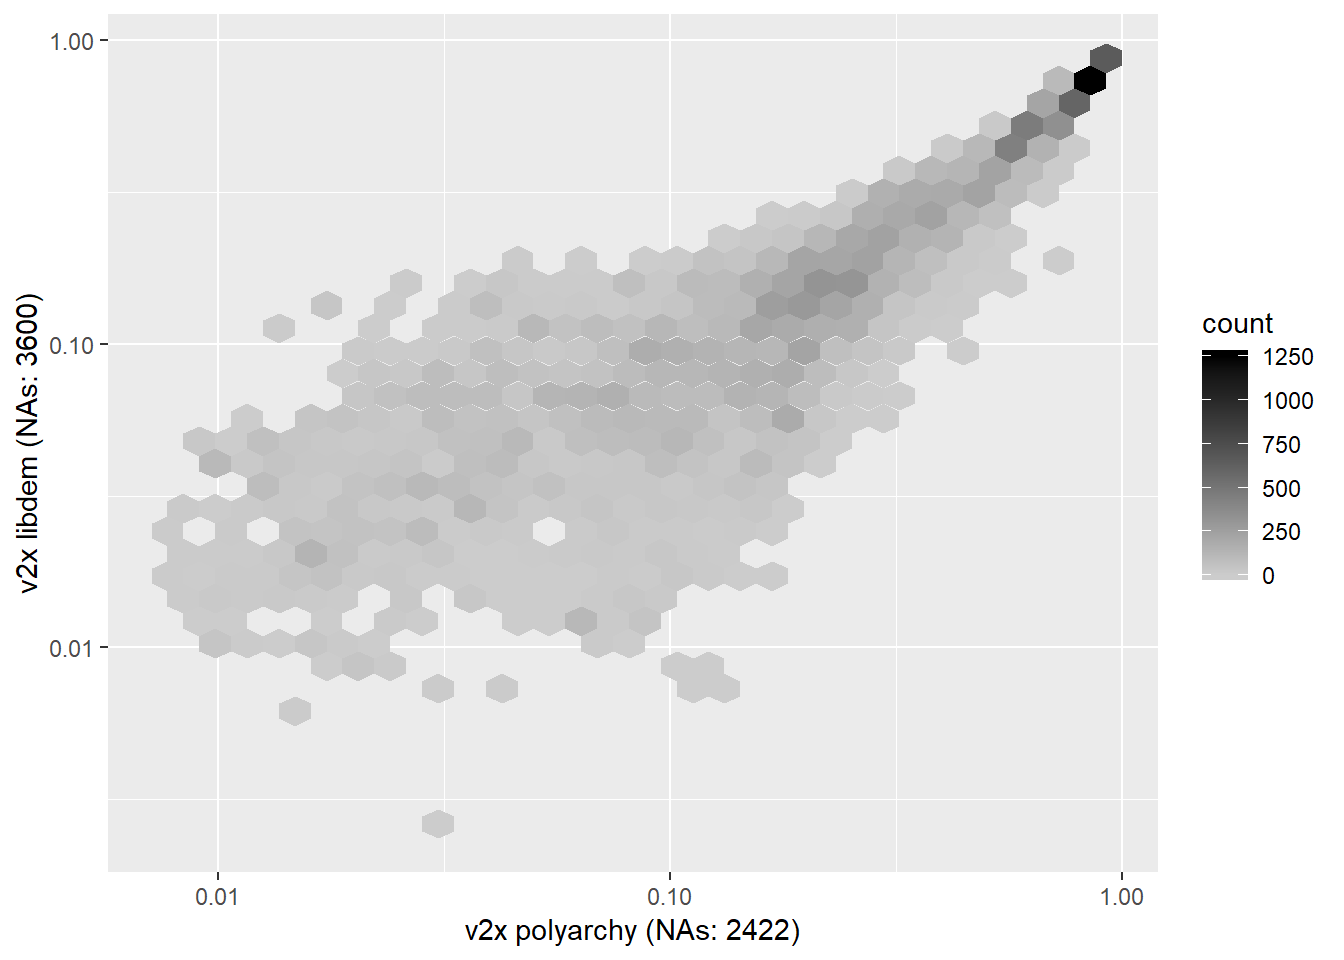
\includegraphics{bachelor-thesis_files/figure-latex/unnamed-chunk-6-1.pdf}

This choice is flexible, as well; should we, for instance, wish to use
the colour aesthetics to represent the year of the observation, the plot
adapts:

\begin{Shaded}
\begin{Highlighting}[]
\NormalTok{df_vdem }\OperatorTok\StringTok{ }
\StringTok{  }\KeywordTok{select}\NormalTok{(v2x_polyarchy, v2x_libdem, year) }\OperatorTok\StringTok{ }
\StringTok{  }\KeywordTok{fx_ggplot}\NormalTok{(}\KeywordTok{aes}\NormalTok{(}\DataTypeTok{x =}\NormalTok{ v2x_polyarchy, }\DataTypeTok{y =}\NormalTok{ v2x_libdem, }\DataTypeTok{colour =}\NormalTok{ year))}
\end{Highlighting}
\end{Shaded}

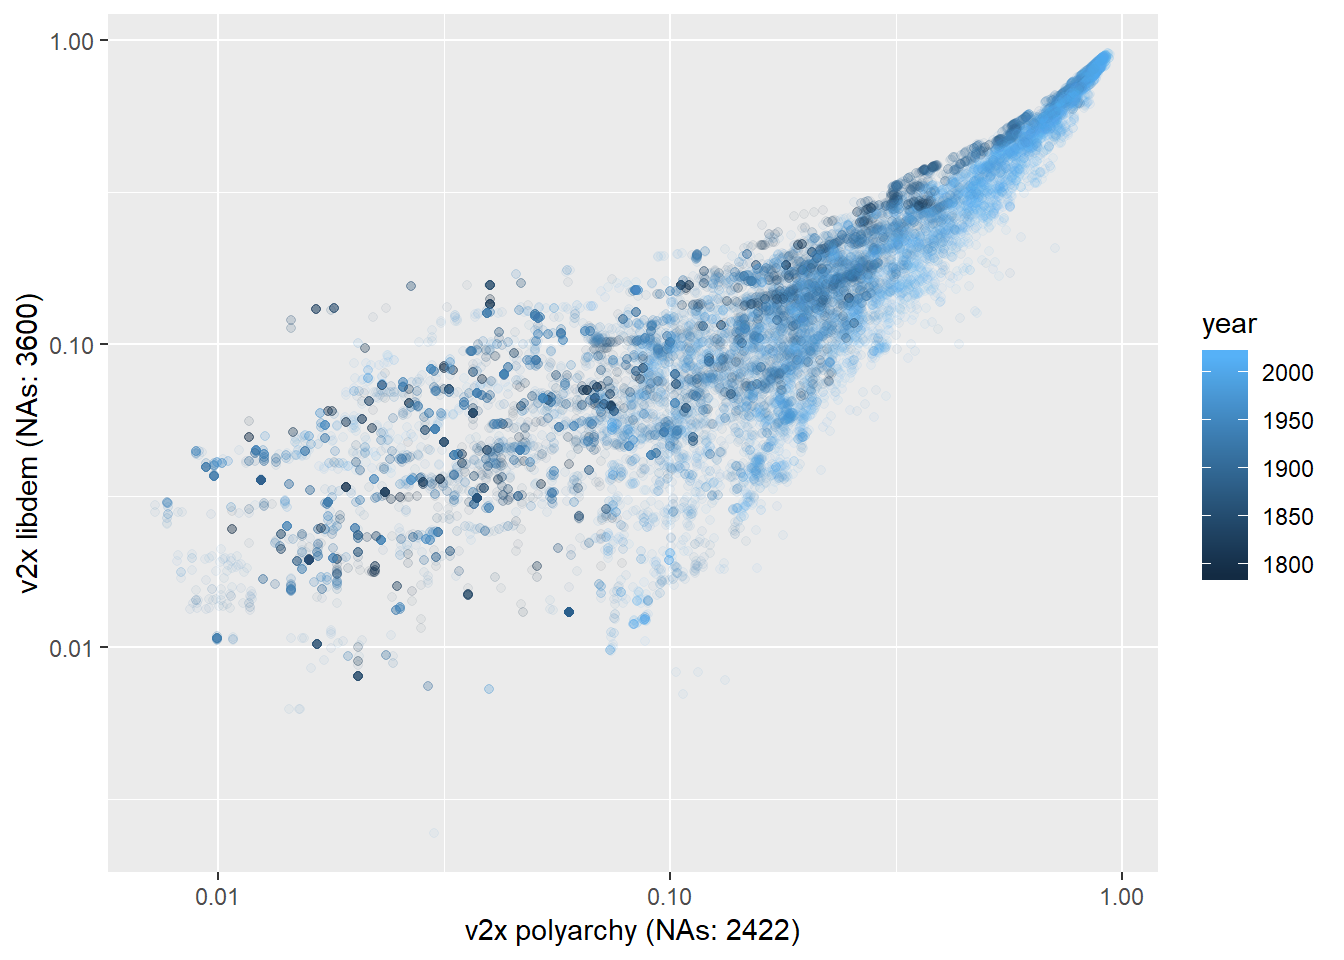
\includegraphics{bachelor-thesis_files/figure-latex/unnamed-chunk-7-1.pdf}

The increased transparency of the points improves oversight over the
plot. Note that \texttt{fx\_ggplot} is not intended to protect the user
from specifications within \texttt{aes} that do not make sense but
rather intends to build the best plot for the specified aesthetics.
Adding the size of the points as an additional aesthetic would render
the plot rather useless. This is, however, not the scope of
\texttt{fx\_ggplot} - I will discuss this point further in chapter 4.

\section{Modifying the default
values}\label{modifying-the-default-values}

The default values which the plot uses may be changed by modifying the
metaframe in which they are stored. Consider, as an example, the
development of the liberal democracy index in Germany and Afghanistan
over time.

\begin{Shaded}
\begin{Highlighting}[]
\NormalTok{df_vdem }\OperatorTok\StringTok{ }
\StringTok{  }\KeywordTok{filter}\NormalTok{(country_name }\OperatorTok\StringTok{ }\KeywordTok{c}\NormalTok{(}\StringTok{"Germany"}\NormalTok{, }\StringTok{"Afghanistan"}\NormalTok{)) }\OperatorTok\StringTok{ }
\StringTok{  }\KeywordTok{select}\NormalTok{(year, v2x_libdem, country_name) }\OperatorTok\StringTok{ }
\StringTok{  }\KeywordTok{fx_ggplot}\NormalTok{(}\KeywordTok{aes}\NormalTok{(}\DataTypeTok{x =}\NormalTok{ year, }\DataTypeTok{y =}\NormalTok{ v2x_libdem, }\DataTypeTok{colour =}\NormalTok{ country_name))}
\end{Highlighting}
\end{Shaded}

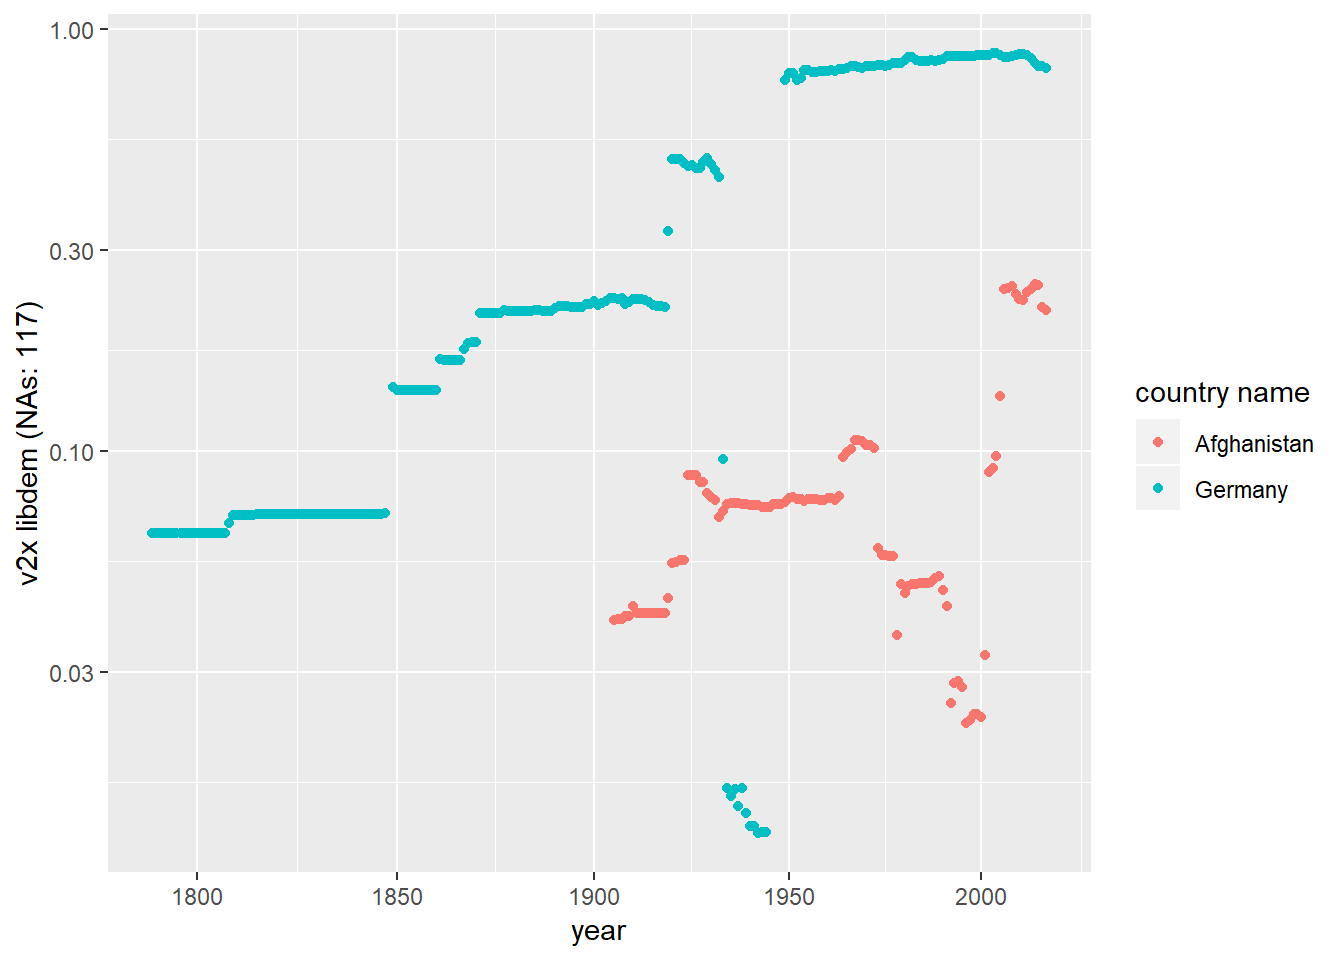
\includegraphics{bachelor-thesis_files/figure-latex/unnamed-chunk-8-1.pdf}

This is evidently not a very useful plot; although we are able to
extrapolate the developments in both countries, a line plot would be
preferred. The problem is that \texttt{fx\_ggplot} does not know that
year represents a time. The fxGeom class corresponding the time variable
is ``Time''. We can modify the metaframe accordingly.

\begin{Shaded}
\begin{Highlighting}[]
\CommentTok{# To modify default values, we need to define a function that changes the fxGeom_class of }
\CommentTok{# the questionable names and returns that (modified or unmodified) argument.}
\NormalTok{year_is_time <-}\StringTok{ }\ControlFlowTok{function}\NormalTok{(fxGeom_class, name) \{}
  \ControlFlowTok{if}\NormalTok{(name }\OperatorTok{==}\StringTok{ "year"}\NormalTok{) }\KeywordTok{return}\NormalTok{(}\StringTok{"Time"}\NormalTok{)}
\NormalTok{  fxGeom_class}
\NormalTok{\}}
\NormalTok{df_vdem }\OperatorTok\StringTok{ }
\StringTok{  }\KeywordTok{filter}\NormalTok{(country_name }\OperatorTok\StringTok{ }\KeywordTok{c}\NormalTok{(}\StringTok{"Germany"}\NormalTok{, }\StringTok{"Afghanistan"}\NormalTok{)) }\OperatorTok\StringTok{ }
\StringTok{  }\KeywordTok{select}\NormalTok{(year, v2x_libdem, country_name) }\OperatorTok\StringTok{ }
\StringTok{  }\CommentTok{# If called without an argument, fx_default simply instantiates the metaframe with the names.}
\StringTok{  }\KeywordTok{fx_default}\NormalTok{() }\OperatorTok\StringTok{ }
\StringTok{  }\CommentTok{# The function responsible for the default value is fx_default_fxGeom_class. }
\StringTok{  }\CommentTok{# It accepts as an argument a function that changes these classes.}
\StringTok{  }\CommentTok{# Its first argument is the data frame itself.}
\StringTok{  }\KeywordTok{mutate_mf}\NormalTok{(}
    \DataTypeTok{fxGeom_class =} \KeywordTok{fx_default_fxGeom_class}\NormalTok{(., }\DataTypeTok{custom_fun =}\NormalTok{ year_is_time), }
    \DataTypeTok{fxGeom_assoc_vars =} \KeywordTok{aes}\NormalTok{(}\DataTypeTok{group =}\NormalTok{ country_name) }
    \CommentTok{# The second variable specifies which observations should be viewed as a instances of a }
    \CommentTok{# coherent unit, i. e. be connected by lines.}
\NormalTok{  ) }\OperatorTok\StringTok{ }
\StringTok{  }\KeywordTok{fx_ggplot}\NormalTok{(}\KeywordTok{aes}\NormalTok{(}\DataTypeTok{x =}\NormalTok{ year, }\DataTypeTok{y =}\NormalTok{ v2x_libdem, }\DataTypeTok{colour =}\NormalTok{ country_name))}
\end{Highlighting}
\end{Shaded}

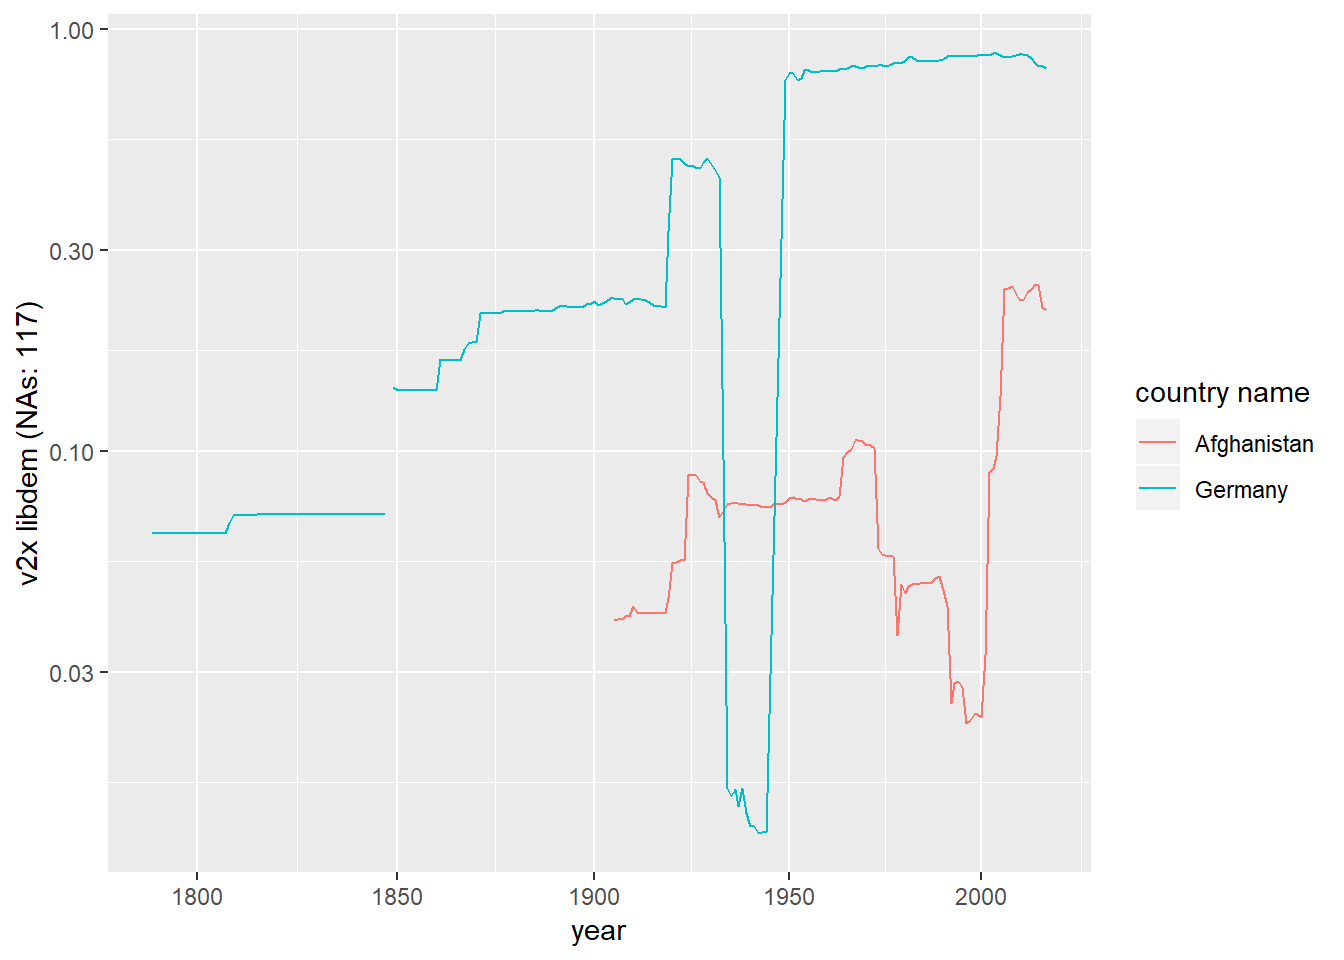
\includegraphics{bachelor-thesis_files/figure-latex/unnamed-chunk-9-1.pdf}

Now, the expected line plot is displayed. The time class is able to
prevent overplotting, as well. Suppose that we now consider all
observations:

\begin{Shaded}
\begin{Highlighting}[]
\NormalTok{df_vdem }\OperatorTok\StringTok{ }
\StringTok{  }\KeywordTok{select}\NormalTok{(year, v2x_libdem, country_name) }\OperatorTok\StringTok{ }
\StringTok{  }\CommentTok{# If called without an argument, fx_default simply instantiates the metaframe with the names.}
\StringTok{  }\KeywordTok{fx_default}\NormalTok{() }\OperatorTok\StringTok{ }
\StringTok{  }\CommentTok{# The function responsible for the default value is fx_default_fxGeom_class. }
\StringTok{  }\CommentTok{# It accepts as an argument a function that changes these classes.}
\StringTok{  }\CommentTok{# Its first argument is the data frame itself.}
\StringTok{  }\KeywordTok{mutate_mf}\NormalTok{(}
    \DataTypeTok{fxGeom_class =} \KeywordTok{fx_default_fxGeom_class}\NormalTok{(., }\DataTypeTok{custom_fun =}\NormalTok{ year_is_time), }
    \DataTypeTok{fxGeom_assoc_vars =}\NormalTok{ purrr}\OperatorTok{::}\KeywordTok{map}\NormalTok{(}
\NormalTok{      name, }
      \ControlFlowTok{function}\NormalTok{(name) \{}
        \ControlFlowTok{if}\NormalTok{(name }\OperatorTok{==}\StringTok{ "year"}\NormalTok{) }\KeywordTok{return}\NormalTok{(}\KeywordTok{aes}\NormalTok{(}\DataTypeTok{group =}\NormalTok{ country_name))}
        \KeywordTok{aes}\NormalTok{()}
\NormalTok{      \}}
\NormalTok{    )}
    \CommentTok{# The second variable specifies which observations should be viewed as a instances of a }
    \CommentTok{# coherent unit, i. e. be connected by lines.}
\NormalTok{  ) }\OperatorTok\StringTok{ }
\StringTok{  }\KeywordTok{fx_ggplot}\NormalTok{(}\KeywordTok{aes}\NormalTok{(}\DataTypeTok{x =}\NormalTok{ year, }\DataTypeTok{y =}\NormalTok{ v2x_libdem))}
\end{Highlighting}
\end{Shaded}

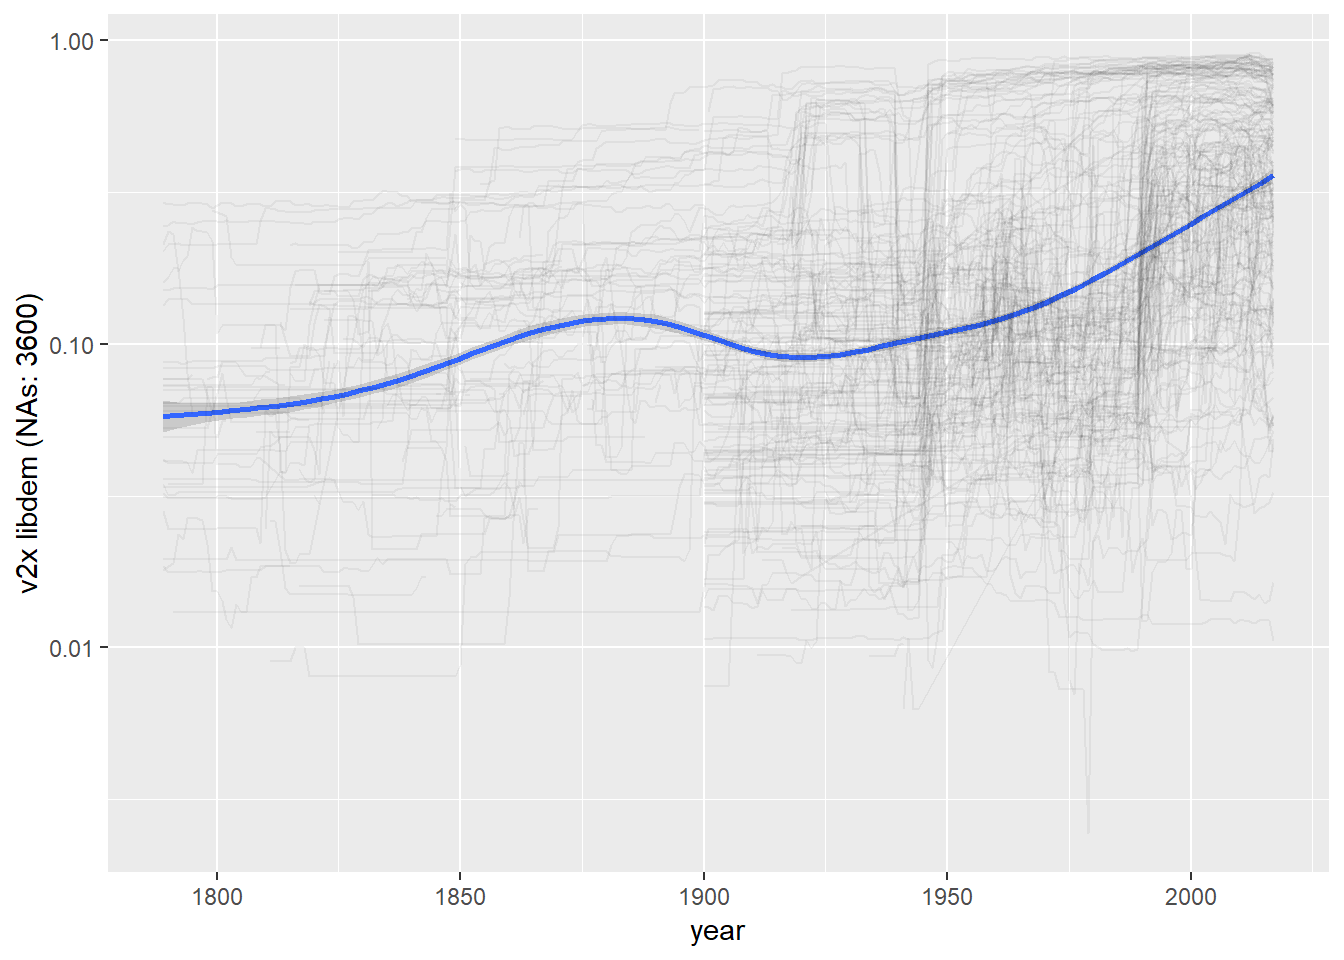
\includegraphics{bachelor-thesis_files/figure-latex/unnamed-chunk-10-1.pdf}

\hypertarget{summary}{\section{Summary}\label{summary}}

The ability to modify the default values is a crucial feature of
\texttt{tectr} and I will discuss the broader background of these
considerations in the next chapter.

At the end of this chapter, let me summarize the depicted workflow:

\begin{itemize}
\item
  at first, we were interested in different visualizations and we
  approximated this by specifying aesthetics
\item
  the first visualizations broadly matched our idea and we saw no need
  to adapt the plots
\item
  as we encountered a plot we were unhappy with, we changed two default
  parameters. We were content with the result once again and the
  modification was both quick and easy to store.
\end{itemize}

This is the essence of \texttt{tectr}'s goal and the considerations in
the subsequent chapter will be a more extensive embedding of the
following two priorities:

\begin{enumerate}
\def\labelenumi{\arabic{enumi}.}
\item
  Implement \emph{strong defaults} which the user needs to change as
  scarcely as possible.
\item
  When the user needs to change something, make it \emph{easy and
  permanent}.
\end{enumerate}

These are, of course, very general principles. When applied to
\texttt{tectr}, however, it becomes evident in what way they would not
be of use in other packages.

Take, for instance, the scale transformations. While they will be
discussed in more detail, below, the default assumes certain
transformations for particularly skewed data. This would be completely
unsuitable in the case of the underlying package \texttt{ggplot2}.
Imputed transformations introduce uncertainty as the user is unsure what
exactly he will produce unless he specifies a lot of parameters. In most
cases \emph{easy defaults} are therefore more sensible than \emph{strong
defaults}. Only the second priority makes them useful; if they could not
reliably and permanently be changed, they would constitute a constant
burden. With these two priorities, however, they are more likely to
fulfill their intended purpose of decreasing the cognitive cost of the
user.

\hypertarget{concept}{\chapter{\texorpdfstring{Description of
\texttt{tectr}}{Description of tectr}}\label{concept}}

\section{Effective Explicitness: A perspective of
knowledge}\label{effective-explicitness-a-perspective-of-knowledge}

Let us revisit the introduction: specified functions and default values
render R a powerful programming language for statistical analysis. These
concepts are so useful because they constitute crystallized knowledge:
when the user calls the function \texttt{read.csv}, he effectively uses
the programmer's knowledge of how to read in csv-files and therefore
lightens his own cognitive load. Of course, this also applies if she has
written the function herself; in this case, by externalizing the
knowledge she does not need to think about the specifics anymore. There
are therefore two main advantages of externalizing knowledge. Other
users benefit from the user's knowledge and the user himself benefits
from its automization.

Normally, these default values cannot be particularly fancy as the user
needs to understand what the function yields under all circumstances --
even if this result is not ideal. This is the restriction that will be
loosened for \texttt{tectr}. The intention behind this is to automize
\emph{more} knowledge.

How does this work? Let us briefly consider a hypothetical statistician
who looks at a dataset. He might at first want to look at the
distribution and a few summary statistics of the variable.
Simultaneously, he learns the name and the definition of a variable. He
might look at relationships between several variables. During all that
time, he will create internal knowledge concerning a proper form of the
statistical summary or a certain visualization, dependent on different
aspects; for instance, he might determine a better axis title than
\texttt{v2x\_polyarchy} or find it helpful to denote the mean of the
variable on the axis. He might also, for instance determine that a line
plot is a better fit than a scatter plot in this case or find that a
certain variable transformation is helpful.

This knowledge is seldomly notated which leads to a less efficient
workflow. After all, this means that while exploring the data, the
statistician will think about every modification of the plot. As a
by-product, any non-crucial change will be left out, even though she
might actually benefit from a more descriptive axis title. More
severely, when she wants to communicate her results, she needs to
reproduce all the internally held knowledge; if she creates a certain
visualization she needs to modify the axis title, in a table describing
the variables, she needs to replace the non-descriptive variable names.
If she would like an interactive visualization of the statistical
analysis, the problem becomes even bigger; in this case, she needs to
externalize her knowledge after the fact.

In order to resolve these issues, \texttt{tectr} attempts to track these
decisions \emph{while they are being made}. The program does that by
asking the user to be \emph{explicit} about his knowledge -- which is
usually only represented internally.

If \texttt{tectr} used default values of a similar kind as other
functions, this would lead to a severe burden on the user as it is time
expensive to externalize knowledge. \texttt{tectr} therefore uses more
flexible default values that attempt to approximate the statistician's
thought process. The user therefore mainly has to intervene when
something does not adhere to canonical assumptions. As he is more likely
to think about these situations explicitly, the burden seems likely to
decrease even considering that under usual circumstances, the users will
be forced to make these explicit decisions several times.

I will call this concept \emph{effective explicitness} and it is central
to \texttt{tectr}. To emphasize that, the keyword guides the semantics
of \texttt{tectr}: those functions and objects which support effective
explicitness will be preceded by \emph{fx} (e\textbf{f}fective
e\textbf{x}plicitness, pronounced: effex).

The notion of explicitness is clear in this context; if the user gains
new knowledge that is not represented in the metaframe he should be
explicit about it. This applies to visualizations as well as general
observations which he may notate in a comments field. This process
should be effective in two ways: firstly, the metaframe needs to imitate
the statistical thought process closely enough that many of its
approximations are valid; secondly, if adaptations need to be made, they
should be scalable. Consider, as an example, they variable year in the
previous chapter. The immediate assumption of the program that this was
an ordinary continuous variable was wrong. In order to correct the
assumptions, it was sufficient to make explicit that the variable
referred to time and tracked the development for different countries. On
the other hand, the variable could also have been so individual that
these little changes would not have sufficed. In these cases, it should
be possible to make broader changes. The remaining chapter will present
a pilot implementation of this more general philosophy. Before going on
to discuss specific functions, I will present the underlying concepts
which power these functions. In order to properly discuss the functions,
I will focus on the following aspects:

\begin{itemize}
\item
  How is communicated what the functions should yield?
\item
  How does the function allow the user to be explicit?
\item
  What would be alternative implementations?
\item
  How mature is the function?
\end{itemize}

The last point is especially important: as a pilot implementation,
\texttt{tectr} provides functionality that seems to go in the right
direction. However, only a combination of more exhaustive features and
applications will determine whether the approach was the right one. It
is therefore important to identify those functions where an entirely
different track of thought might be necessary in the future. In order to
make the description lightweight and not focus too much on the
particularities of implementation, I will often refer to the package
documentation for further information.

\section{Underlying structure}\label{underlying-structure}

\subsection{The metaframe}\label{the-metaframe}

The \emph{metaframe} is the attribute of a database which captures the
knowledge of the user. It adheres to the principle of tidy data
\citep{Wickham2014}:

\begin{quote}
Each variable forms a column.

Each observation forms a row.

Each type of observational unit forms a table.
\end{quote}

Clearly, additional information about observations can be stored in an
additional column. The metaframe stores additional information about
variables by treating every variable as an observation and every type of
information as a column. It consists of different protected variable
names that fulfill specific functions. The \texttt{name} column refers
to the corresponding variable name. The remaining information is
preceded by a keyword to make clear what the variable refers to. More
specifically, those variables that refer to semantic information are
preceded by \texttt{fxInfo} (e. g. the name of variable
\texttt{fxInfo\_name}) and those variables that give information on the
visualization are preceded by \texttt{fxGeom}.

For details on metaframes, how to set or change them see the
documentation. In my opinion the best workflow is provided by
instantiating the metaframe with \texttt{fx\_default} and then adding
columns via \texttt{mutate\_mf}. This allows you to only use the data
frame itself as an attribute and provides a concise terminology:

\begin{Shaded}
\begin{Highlighting}[]
\NormalTok{data <-}\StringTok{ }
\StringTok{  }\KeywordTok{tibble}\NormalTok{(}\DataTypeTok{ht =} \KeywordTok{c}\NormalTok{(}\DecValTok{158}\NormalTok{, }\DecValTok{189}\NormalTok{, }\DecValTok{178}\NormalTok{)) }\OperatorTok\StringTok{ }
\StringTok{  }\KeywordTok{fx_default}\NormalTok{() }\OperatorTok\StringTok{ }
\StringTok{  }\KeywordTok{mutate_mf}\NormalTok{(}\DataTypeTok{fxInfo_name =} \StringTok{"Height"}\NormalTok{)}
\KeywordTok{metaframe}\NormalTok{(data)}
\end{Highlighting}
\end{Shaded}

\begin{verbatim}
##   name fxInfo_name
## 1   ht      Height
\end{verbatim}

\subsection{Extending fx functions}\label{extending-fx-functions}

\subsubsection{Dispatch}\label{dispatch}

Whereas in most cases, modifying the parameters to the functions should
be sufficient, there are also many applications where a more extensive
modification is necessary -- or at least more effective. \texttt{tectr}
uses method dispatch to structure these extension. In certain occasions,
S4 classes are necessary. As long as S3 class suffice, they are
utilized.

It is important to emphasize that the fx function themselves are not
generics. Internally, every fx function calls an \texttt{fxi} (short for
fx \emph{internal}) function which modifies its arguments to make
dispatch possible. I will elaborate on the particular mechanism in the
following sections. By defining dummy classes, the calls to so called
\texttt{fxe} (short for fx \emph{extendible}) functions employ dispatch
and can be extended. The metaframe information of the current variable
is called as spliced input to the \texttt{fxe} function. For instance,
in the example above, an extendible function \texttt{fxe\_fun} would
have received as additional input the argument \texttt{fxInfo\_name} and
\texttt{name}.

\subsubsection{S3 dummy classes}\label{s3-dummy-classes}

S3 dummy classes are mainly powered by the function \texttt{fxd} which
creates a \emph{subclass} for a specific \emph{task}. For instance, the
task ``default'' which specifies the default values for the metaframe
columns has as its subclasses the corresponding columns, e. g.:

\begin{Shaded}
\begin{Highlighting}[]
\KeywordTok{fxd}\NormalTok{(}\StringTok{"default"}\NormalTok{, }\StringTok{"fxInfo_name"}\NormalTok{)}
\end{Highlighting}
\end{Shaded}

\begin{verbatim}
## list()
## attr(,"class")
## [1] "fxd_default_fxInfo_name" "fxd_default"            
## [3] "fxd"
\end{verbatim}

This provides a lightweight and effective mechanism for dispatch via
dummy classes.

\subsubsection{S4 dummy classes}\label{s4-dummy-classes}

S4 dummy classes are powered by different classes for every task they
employ. For instance the \texttt{fxGeom} dummy classes all inherit from
\texttt{fxGeom} and consist of the aforementioned possible classes of
input to visualization. Consider, for instance,

\begin{Shaded}
\begin{Highlighting}[]
\KeywordTok{fxGeom}\NormalTok{(}\StringTok{"Continuous"}\NormalTok{)}
\end{Highlighting}
\end{Shaded}

\begin{verbatim}
## An object of class "fxGeomContinuous"
## [1] "Continuous"
\end{verbatim}

which yields the corresponding S4 class \texttt{fxGeomContinuous}.

This mechanism provides a better overview over all possible classes.
However, it is necessary to explicitly define every task and every
subclass. Normally, the \texttt{fxd} mechanism should be preferred. S4
dummy classes are mainly employed when multiple dispatch becomes
necessary, see \texttt{fx\_ggplot}.

\subsection{Other concepts}\label{other-concepts}

I have defined a few other objects that come in useful. I will shortly
elaborate on them here.

\subsubsection{Filepaths}\label{filepaths}

The S3 class \texttt{filepath} consists of a character vector which
contains paths to external data and a \texttt{reader} attribute which
can read in the data. It allows you to retrieve stored data within a
metaframe in an uncomplicated way.

\subsubsection{fx factors}\label{fx-factors}

fx factors are a very simple class which extends the concept of factors
from \texttt{character}s to arbitrary classes. Certain columns of the
metaframe might, for instance, contain different functions many times
and it would be a waste to store them separately. \texttt{fx\_factor}
creates an object which has as the attribute levels its unique values
and refers to them within every element via the index of the levels. The
original object can be recreated via \texttt{fx\_evaluate}.

\section{\texorpdfstring{\texttt{fx\_default}}{fx\_default}}\label{fx_default}

\subsection{General purpose}\label{general-purpose}

\texttt{fx\_default} computes default values for every column of the
metaframe so that the different fx functions can fill up the metaframe
with the remaining necessary columns. The function therefore uses
specific heuristics for the different columns to infer sensible values.
As in many cases, the default values are modified, for every column
there is a function
\texttt{fx\_default\_\textless{}colname\textgreater{}} (e. g.
\texttt{fx\_default\_fxInfo\_name}) which allows the user to access the
default values separate from the internal mechanism of
\texttt{fx\_default}.

A call to \texttt{fx\_default} specifies the columns to be imputed. By
default, if the data frame has not metaframe, it creates the metaframe
with one observation for every variable name.

\subsection{Extensions}\label{extensions}

Extensions can be provided via S3 method dispatch over the function
\texttt{fxe\_default} and the class
\texttt{fxd\_default\_\textless{}colname\textgreater{}}. The function
may depend on the data and on its metaframe. If possible, it is
recommended that the functions only depend on the data frame and the
name column of the metaframe. Consider, for instance, the default
function for \texttt{fxGeom\_class}:

\begin{Shaded}
\begin{Highlighting}[]
\NormalTok{tectr}\OperatorTok{:::}\NormalTok{fxe_default.fxd_default_fxGeom_class}
\end{Highlighting}
\end{Shaded}

\begin{verbatim}
## function(data, mf, col, ...)
##   fx_default_fxGeom_class(data, mf)
## <bytecode: 0x00000000462c01a8>
## <environment: namespace:tectr>
\end{verbatim}

Internally, it calls the more accessible function
\texttt{fx\_default\_fxGeom\_class} which does the work
(\href{\%60fx_ggplot\%60}{\#fx-ggplot} will explain how the default
value is determined).

\subsection{Alternative
implementations}\label{alternative-implementations}

As with default values in functions in R, there are essentially two
possible implementations: either the default is specified in the head or
the function recognizes that the default is needed if the argument has
the value \texttt{NULL}. Which mechanism is preferable, depends strongly
on the context. It is recommended that parameters that are specific to
one function and have a very simple default value (for instance, a
constant numerical value) are marked via \texttt{NULL} whereas broadly
applicable parameters that employ a more elaborate inference mechanism
may be of use for the user and should therefore be implemented via an
\texttt{fx\_default} function.

\subsection{Lifecycle}\label{lifecycle}

The purpose of \texttt{fx\_default} is clearly outlined and its
application is very simple. Modifications of the internal dispatch are
possible but the extendible functions and \texttt{fx\_default} itself
are unlikely to be reworked.

\section{\texorpdfstring{\texttt{fx\_info}}{fx\_info}}\label{fx_info}

\subsection{General purpose}\label{general-purpose-1}

This function provides information on the different variables to the
user. Examples for this information would be

\begin{itemize}
\tightlist
\item
  the name of the variable which differs from its internal name
\item
  the description or definition of the variable
\item
  summary statistics.
\end{itemize}

A call to \texttt{fx\_info} consists of the data itself, a topic and
potentially additional parameters. The \emph{topic} may either be a
certain semantic topic like the name or the description or it may invoke
a specific method. The most useful example of a topic is ``stats'' which
renders a summary table with descriptive statistics that can be
specified in the argument statistics:

\begin{Shaded}
\begin{Highlighting}[]
\KeywordTok{fx_info}\NormalTok{(mtcars, }\StringTok{"stats"}\NormalTok{, }\DataTypeTok{statistics =} \KeywordTok{c}\NormalTok{(}\StringTok{"mean"}\NormalTok{, }\StringTok{"quantile"}\NormalTok{))}
\end{Highlighting}
\end{Shaded}

\begin{verbatim}
## # A tibble: 11 x 7
##    name     mean `quantile: 0%` `quantile: 25%` `quantile: 50%`
##    <chr>   <dbl>          <dbl>           <dbl>           <dbl>
##  1 mpg    20.1            10.4            15.4            19.2 
##  2 cyl     6.19            4               4               6   
##  3 disp  231.             71.1           121.            196.  
##  4 hp    147.             52              96.5           123   
##  5 drat    3.60            2.76            3.08            3.70
##  6 wt      3.22            1.51            2.58            3.32
##  7 qsec   17.8            14.5            16.9            17.7 
##  8 vs      0.438           0               0               0   
##  9 am      0.406           0               0               0   
## 10 gear    3.69            3               3               4   
## 11 carb    2.81            1               2               2   
## # ... with 2 more variables: `quantile: 75%` <dbl>, `quantile: 100%` <dbl>
\end{verbatim}

As can be seen the function returns a data frame with a certain
information in every column. If no method for the particular topic
exists, the function searches the metaframe for a column of the name
``fxInfo\_'' and returns that. Consider, for instance, a name and a
short comment:

\begin{Shaded}
\begin{Highlighting}[]
\NormalTok{mtcars }\OperatorTok\StringTok{ }
\StringTok{  }\KeywordTok{select}\NormalTok{(mpg) }\OperatorTok\StringTok{ }
\StringTok{  }\KeywordTok{fx_default}\NormalTok{() }\OperatorTok\StringTok{ }
\StringTok{  }\KeywordTok{mutate_mf}\NormalTok{(}
    \DataTypeTok{fxInfo_name =} \StringTok{"Miles/(US) gallon"}\NormalTok{, }
    \DataTypeTok{fxInfo_comment =} \StringTok{"A gallon is 3.79 litres."}
\NormalTok{  ) }\OperatorTok\StringTok{ }
\StringTok{  }\KeywordTok{fx_info}\NormalTok{(}\KeywordTok{c}\NormalTok{(}\StringTok{"name"}\NormalTok{, }\StringTok{"comment"}\NormalTok{, }\StringTok{"stats"}\NormalTok{), }\DataTypeTok{statistics =} \KeywordTok{c}\NormalTok{(}\StringTok{"mean"}\NormalTok{, }\StringTok{"quantile"}\NormalTok{))}
\end{Highlighting}
\end{Shaded}

\begin{verbatim}
## # A tibble: 1 x 9
##   name  Name  Comment  mean `quantile: 0%` `quantile: 25%` `quantile: 50%`
##   <chr> <chr> <chr>   <dbl>          <dbl>           <dbl>           <dbl>
## 1 mpg   Mile~ A gall~  20.1           10.4            15.4            19.2
## # ... with 2 more variables: `quantile: 75%` <dbl>, `quantile: 100%` <dbl>
\end{verbatim}

We will later use this functionality to create meaningful descriptive
tables.

You may provide either characters or functions to statistics. Characters
are evaluated via \texttt{do.call}, functions are called directly. If
you specify a function, you should allow for arbitrary parameters via
\texttt{...} as a function will receive the columns of the metaframe as
input. A function's first argument should be the corresponding column of
the data frame. Consider the following example:

\begin{Shaded}
\begin{Highlighting}[]
\NormalTok{stat_mean <-}\StringTok{ }\ControlFlowTok{function}\NormalTok{(x, ..., fxInfo_digits) }
\NormalTok{  x }\OperatorTok\StringTok{ }\KeywordTok{mean}\NormalTok{() }\OperatorTok\StringTok{ }\KeywordTok{round}\NormalTok{(}\DataTypeTok{digits =}\NormalTok{ fxInfo_digits)}
\NormalTok{mtcars }\OperatorTok\StringTok{ }
\StringTok{  }\KeywordTok{select}\NormalTok{(mpg) }\OperatorTok\StringTok{ }
\StringTok{  }\KeywordTok{fx_default}\NormalTok{() }\OperatorTok\StringTok{ }
\StringTok{  }\KeywordTok{mutate_mf}\NormalTok{(}
    \DataTypeTok{fxInfo_name =} \StringTok{"Miles/(US) gallon"}\NormalTok{, }
    \DataTypeTok{fxInfo_digits =} \DecValTok{3}
\NormalTok{  ) }\OperatorTok\StringTok{ }
\StringTok{  }\KeywordTok{fx_info}\NormalTok{(}\KeywordTok{c}\NormalTok{(}\StringTok{"name"}\NormalTok{, }\StringTok{"stats"}\NormalTok{), }
          \DataTypeTok{statistics =} \KeywordTok{list}\NormalTok{(}\DataTypeTok{mean =}\NormalTok{ stat_mean))}
\end{Highlighting}
\end{Shaded}

\begin{verbatim}
## # A tibble: 1 x 3
##   name  Name               mean
##   <chr> <chr>             <dbl>
## 1 mpg   Miles/(US) gallon  20.1
\end{verbatim}

\subsection{Extensions}\label{extensions-1}

Extensions can be provide via dispatch over \texttt{fxe\_info}. The
dummy class for a certain topic will be provided by
\texttt{fxd("info",\ \textless{}topic\textgreater{})}, e. g.

\begin{Shaded}
\begin{Highlighting}[]
\KeywordTok{fxd}\NormalTok{(}\StringTok{"info"}\NormalTok{, }\StringTok{"stats"}\NormalTok{)}
\end{Highlighting}
\end{Shaded}

\begin{verbatim}
## list()
## attr(,"class")
## [1] "fxd_info_stats" "fxd_info"       "fxd"
\end{verbatim}

\subsection{Lifecycle}\label{lifecycle-1}

In my opinion, the combination of simplicity and power makes
\texttt{fx\_info} a very useful function that will most likely retain
its structure. This means that new functions which enhance the power of
\texttt{fx\_info} and especially its stats will be the next step in its
development.

\section{\texorpdfstring{\texttt{fx\_output}}{fx\_output}}\label{fx_output}

\subsection{General purpose}\label{general-purpose-2}

This function makes \texttt{fx\_info} immediately applicable in a wide
variety of applications. It renders the data frame returned by
\texttt{fx\_info} into a certain \emph{form}. In this case, a sparse
wrapper around a function from another package often suffices.
\texttt{fx\_info} may return different formats. Currently, the supported
formats are rst, html, latex and markdown. The two most useful forms
that have been implemented so far are \emph{table} and \emph{collapse}.

As an example, we will consider the mtcars summary statistics:

\begin{Shaded}
\begin{Highlighting}[]
\NormalTok{stat_median <-}\StringTok{ }\ControlFlowTok{function}\NormalTok{(x, ...) }
\NormalTok{  x }\OperatorTok\StringTok{ }\KeywordTok{median}\NormalTok{() }\OperatorTok\StringTok{ }\KeywordTok{round}\NormalTok{(}\DataTypeTok{digits =} \DecValTok{3}\NormalTok{)}
\NormalTok{stat_mean <-}\StringTok{ }\ControlFlowTok{function}\NormalTok{(x, ...)}
\NormalTok{  x }\OperatorTok\StringTok{ }\KeywordTok{mean}\NormalTok{() }\OperatorTok\StringTok{ }\KeywordTok{round}\NormalTok{(}\DataTypeTok{digits =} \DecValTok{3}\NormalTok{)}
\NormalTok{info <-}\StringTok{ }
\StringTok{  }\NormalTok{mtcars }\OperatorTok\StringTok{ }
\StringTok{  }\KeywordTok{fx_info}\NormalTok{(}\StringTok{"stats"}\NormalTok{, }\KeywordTok{list}\NormalTok{(}\DataTypeTok{mean =}\NormalTok{ stat_mean, }\DataTypeTok{median =}\NormalTok{ stat_median))}
\NormalTok{info}
\end{Highlighting}
\end{Shaded}

\begin{verbatim}
## # A tibble: 11 x 3
##    name     mean median
##    <chr>   <dbl>  <dbl>
##  1 mpg    20.1    19.2 
##  2 cyl     6.19    6   
##  3 disp  231.    196.  
##  4 hp    147.    123   
##  5 drat    3.60    3.70
##  6 wt      3.22    3.32
##  7 qsec   17.8    17.7 
##  8 vs      0.438   0   
##  9 am      0.406   0   
## 10 gear    3.69    4   
## 11 carb    2.81    2
\end{verbatim}

\begin{Shaded}
\begin{Highlighting}[]
\KeywordTok{fx_output}\NormalTok{(info, }\DataTypeTok{form =} \StringTok{"table"}\NormalTok{, }\DataTypeTok{out_format =} \StringTok{"markdown"}\NormalTok{)}
\end{Highlighting}
\end{Shaded}

\begin{longtable}[]{@{}lrr@{}}
\toprule
name & mean & median\tabularnewline
\midrule
\endhead
mpg & 20.09 & 19.20\tabularnewline
cyl & 6.19 & 6.00\tabularnewline
disp & 230.72 & 196.30\tabularnewline
hp & 146.69 & 123.00\tabularnewline
drat & 3.60 & 3.69\tabularnewline
wt & 3.22 & 3.33\tabularnewline
qsec & 17.85 & 17.71\tabularnewline
vs & 0.44 & 0.00\tabularnewline
am & 0.41 & 0.00\tabularnewline
gear & 3.69 & 4.00\tabularnewline
carb & 2.81 & 2.00\tabularnewline
\bottomrule
\end{longtable}

The form ``collapse'', on the other hand yields one row per observation.
This row consists of different cells in which the variable information
and its name are listed in a specified format and which are then glued
together:

\begin{Shaded}
\begin{Highlighting}[]
\KeywordTok{fx_output}\NormalTok{(info, }\DataTypeTok{form =} \StringTok{"collapse"}\NormalTok{)}
\end{Highlighting}
\end{Shaded}

\begin{verbatim}
## mean:  20.09, median:  19.2
## mean:   6.19, median:   6.0
## mean: 230.72, median: 196.3
## mean: 146.69, median: 123.0
## mean:   3.60, median:   3.7
## mean:   3.22, median:   3.3
## mean:  17.85, median:  17.7
## mean:   0.44, median:   0.0
## mean:   0.41, median:   0.0
## mean:   3.69, median:   4.0
## mean:   2.81, median:   2.0
\end{verbatim}

These specifications can also be modified:

\begin{Shaded}
\begin{Highlighting}[]
\KeywordTok{fx_output}\NormalTok{(info, }\DataTypeTok{form =} \StringTok{"collapse"}\NormalTok{, }\DataTypeTok{cell_scheme =} \StringTok{"The \{name\} is \{value\}."}\NormalTok{, }\DataTypeTok{cell_sep =} \StringTok{" --- "}\NormalTok{)}
\end{Highlighting}
\end{Shaded}

\begin{verbatim}
## The mean is  20.09. --- The median is  19.2.
## The mean is   6.19. --- The median is   6.0.
## The mean is 230.72. --- The median is 196.3.
## The mean is 146.69. --- The median is 123.0.
## The mean is   3.60. --- The median is   3.7.
## The mean is   3.22. --- The median is   3.3.
## The mean is  17.85. --- The median is  17.7.
## The mean is   0.44. --- The median is   0.0.
## The mean is   0.41. --- The median is   0.0.
## The mean is   3.69. --- The median is   4.0.
## The mean is   2.81. --- The median is   2.0.
\end{verbatim}

Further information can be found in the documentation.

\subsection{Extensions}\label{extensions-2}

\texttt{fx\_output} may be extended via the \texttt{fxd} dummy class
with the topic ``output''.

\subsection{Lifecycle}\label{lifecycle-2}

\texttt{fx\_output} is stable and the next step will be to refine and
extend the output forms. In particular, the next version will provide an
output form ``report'' which creates a dynamical report of the kind
which we will render in the \href{fifth\%20chapter}{\#application}.

\section{\texorpdfstring{\texttt{fx\_write}}{fx\_write}}\label{fx_write}

\subsection{General purpose}\label{general-purpose-3}

Besides providing summary tables, the main purpose of \texttt{fx\_info}
is to make information about the variable accessible. The foundation of
this information can often be imported from a codebook of some form (see
the \href{application}{\#application}). Adding and editing this
information -- e. g. correcting typos -- is, however, an awkward
endeavour in R. A text editor of some sort would be more suitable. The
\texttt{fx\_write} family of functions attempts to adress this by
allowing you to export the semantic data to human-readable documents
which can then be modified. As it returns the data frame with a
\texttt{filepath} column which refers to the export file, it can be
easily read in -- this functionality is provided by \texttt{fx\_read}.

Currently, only one \texttt{fx\_write} function is implemented:
\texttt{fx\_write\_json}. This function creates several files in
JavaScript Object Notation which is well readable by humans. The
function is powered by the package \texttt{jsonlite} \citep{jsonlite}
which uses a class based mapping to convert between JSON data and R
objects. For details, see the documentation and the fifth chapter.

\subsection{Extensions}\label{extensions-3}

While \texttt{fx\_write} does not employ any kind of dispatch but is a
family of functions, it can be extended (in a looser definition of the
word) by providing a new method with a consistent interface
\texttt{fx\_write\_\textless{}format\textgreater{}}.

\subsection{Alternative
implementations}\label{alternative-implementations-1}

\texttt{fx\_write} is currently an experimental feature which has its
disadvantages. Most notably, it is difficult to change the codebook
import after somebody has changed the output of this process (i. e. the
exported files). While version control would make this simpler, the fact
remains that all changes to the document would have to be manually
reentered. A primitive editor within R which tracks changes would render
the process more reproducible and less complicated. However, this would
be a considerable effort with limited applicability and for the time
being, it seems to me that a method as represented by
\texttt{fx\_write\_json} (or possibly another format) represents the
best alternative.

\subsection{Lifecycle}\label{lifecycle-3}

This function is at the moment very unstable and should be used with
caution.

\section{\texorpdfstring{\texttt{fx\_ggplot}}{fx\_ggplot}}\label{fx-ggplot}

At last, I present the fx function which has the most extensive
implementation so far: \texttt{fx\_ggplot} which is concerned with the
visualization of the data frame. This functions makes a more extensive
introduction necessary. The first section will discuss the general
concept behind \texttt{fx\_ggplot}. We will then discuss the
implementation in \texttt{tectr} and how it may be extended. The fourth
section discusse3s possible alternatives and the fifth section
elaborates how development of the function will progress.

\subsection{\texorpdfstring{Concept of
\texttt{fx\_ggplot}}{Concept of fx\_ggplot}}\label{concept-of-fx_ggplot}

This function intends to provide a flexible visualization. As an input,
it accepts aesthetics and then attempts to provide the best
visualization that is compatible with the specified aesthetics.
Therefore, it does not answer the question ``What should I know about
these five variables?''. More specifically, it does not prevent you from
overplotting, non-sensical aesthetics etc. In my opinion, it is best
applied by a person who approximately knows what she wants. In this
case, it is especially adept at flexible, interactive visualizations
(see below). For instance, if a statistician is interested in several
time series of different variables, these should be differently
visualized depending on the available information.

While I will discuss this concept below, I will assume, for now, that
this method is valid and consider the following question: How do we
infer the best visualization from a given set of variables? As the
function is created within the syntax of \texttt{ggplot2}, our task is
to infer the set of layers which constructs the plot. These layers fall
in two categories: \emph{dependent} and \emph{independent} layers.

\textbf{Independent} layers will be added for a certain specified
aesthetics regardless of the other aesthetics. An example would be the x
axis title. This title only depends on the x aesthetic. The y aesthetic
has no influence on this layer.

On the other hand, the y aesthetic has a big influence on the question
what geometry we should add, as the suitable geometry depends on all
aesthetics. Such layers are therefore called \textbf{dependent layers}.

The determination of independent layers is relatively clear and simple;
it only depends on one aesthetic and it is therefore easy to define a
function which depends on certain parameters of the variable and yields
a layer. On the other hand, the determination of dependent layers is
messier, as we will se shortly.

For that purpose, I will first present the original concept I had
implemented for dependent layers: a strictly rule based structure which
specifies, for any combination of relevant aesthetics which layers this
would yield. For instance, this structure included:

\begin{itemize}
\tightlist
\item
  continuous x-variable and continuous y-variable:
  \texttt{geom\_point()}
\item
  discrete x-variable and continuous y-variable:
  \texttt{geom\_boxplot()}
\end{itemize}

The basic plots are easily produced with such a system but whereas it
allows the user to be very explicit, it is very difficult to implement a
meaningful influence via parameters. Instead, any new kind of
visualization made necessary an entirely new class with a wide variety
of methods. Furthermore, despite the seeming clarity of these simple
rules, the resulting massive dispatch was likely to end in a lot of
confusion and an unmanageable code base.

I have therefore developed an alternative approach which implements a
voting system for the dependent layers. As a brief overview this process
consists of three phases:

\begin{itemize}
\tightlist
\item
  In the \textbf{nomination phase}, every variable nominates possible
  sets of layers which would make sense with this variable. These
  nominations depend on the aesthetic, the \texttt{fxGeom\_class} and
  possibly the metaframe parameters.
\item
  In the \textbf{veto phase}, every variable receives the entire list of
  nominations and removes those, it is incompatible with.
\item
  In the \textbf{voting phase}, every variable distributes a number of
  votes on the various remaining nominations. These votes depend on
  properties of the nominations. The nomination with the most votes is
  chosen as the winner and yields the dependent layers.
\end{itemize}

This approach may appear unconventional, at first, and I will adress
some counterarguments below. But before that, I will present the
implementation and process of extension for both the independent and the
dependent layers. I will elaborate on the implementation of the
independent layers in the fourth subsection.

I will introduce the implementation with a simple example from the
diamonds dataset: we will consider as \texttt{x} aesthetic the weight in
\texttt{carat} and as \texttt{y} aesthetic the \texttt{price}. In the
end, we will have created the following plot:

\begin{Shaded}
\begin{Highlighting}[]
\KeywordTok{fx_ggplot}\NormalTok{(diamonds, }\KeywordTok{aes}\NormalTok{(}\DataTypeTok{x =}\NormalTok{ carat, }\DataTypeTok{y =}\NormalTok{ price))}
\end{Highlighting}
\end{Shaded}

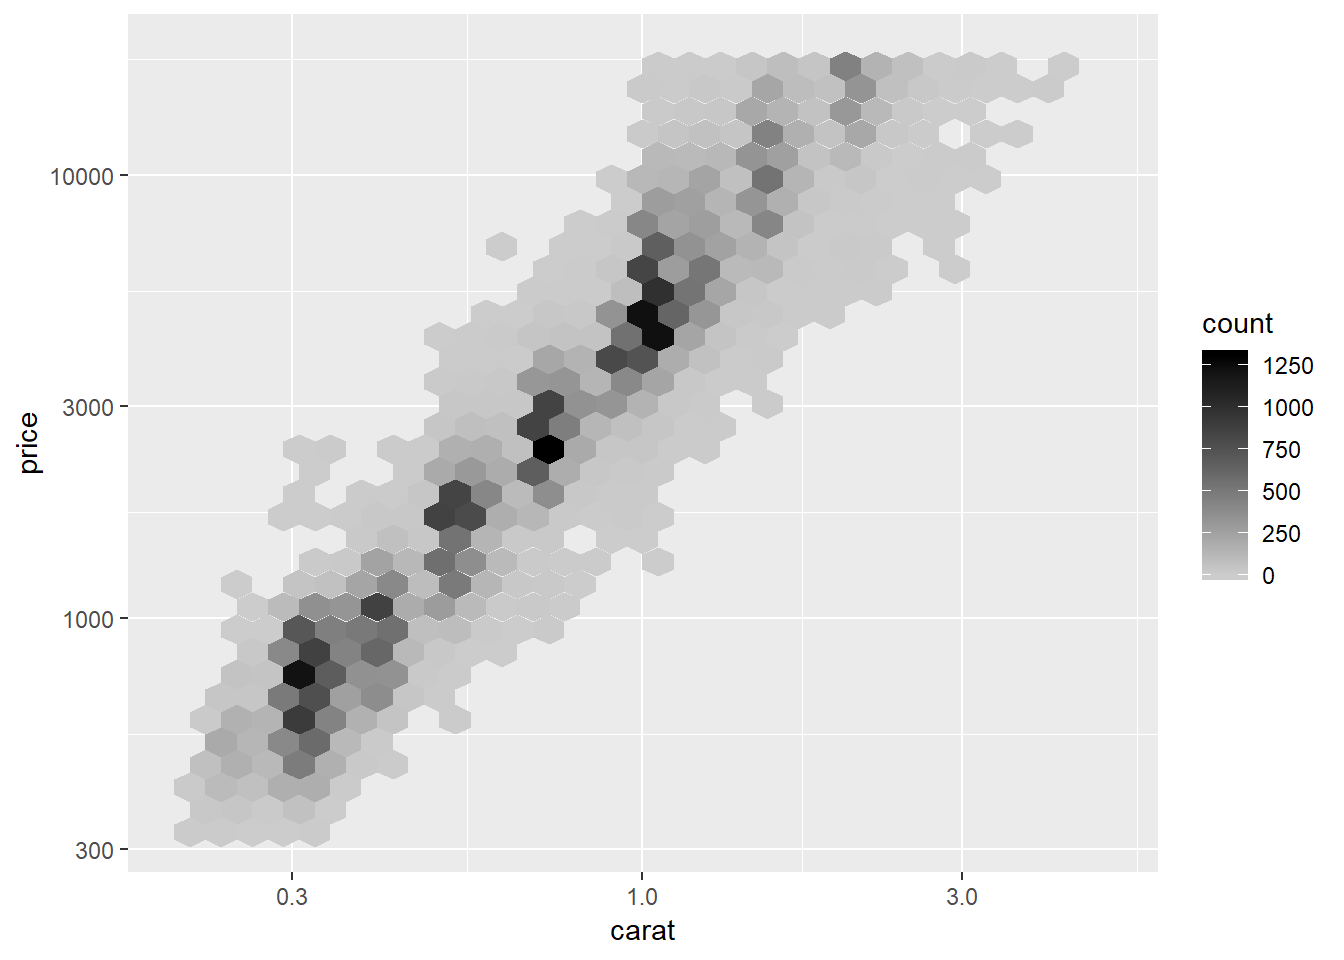
\includegraphics{bachelor-thesis_files/figure-latex/unnamed-chunk-23-1.pdf}

The first step is to infer the default values of the metaframe. All
required columns for \texttt{fx\_ggplot} are stored in the vector
\texttt{fx\_ggplot\_columns}:

\begin{Shaded}
\begin{Highlighting}[]
\NormalTok{fx_diamonds <-}\StringTok{ }
\StringTok{  }\NormalTok{diamonds }\OperatorTok\StringTok{ }
\StringTok{  }\KeywordTok{select}\NormalTok{(carat, price) }\OperatorTok\StringTok{ }
\StringTok{  }\KeywordTok{fx_default}\NormalTok{(}\DataTypeTok{columns =}\NormalTok{ fx_ggplot_columns)}
\KeywordTok{metaframe}\NormalTok{(fx_diamonds) }\OperatorTok\StringTok{ }
\StringTok{  }\KeywordTok{kable}\NormalTok{() }\OperatorTok\StringTok{ }
\StringTok{  }\NormalTok{kableExtra}\OperatorTok{::}\KeywordTok{kable_styling}\NormalTok{()}
\end{Highlighting}
\end{Shaded}

name

fxGeom\_class

fxGeom\_limits

fxGeom\_trans

fxInfo\_name

carat

Continuous

c(0.2, 5.01)

log10

carat

price

Continuous

c(326, 18823)

log10

price

\subsection{Implementation of the independent
layers}\label{implementation-of-the-independent-layers}

The independent layers are determined by the internal function
\texttt{fxi\_layer\_single} which calls \texttt{fxe\_layer\_single} for
every aesthetic. This function dispatches over \texttt{fx\_geom}, the
argument that is created by the \texttt{fxGeom\_class} column.
Therefore, the function is once called for the class
\texttt{fxGeomContinuous} and \texttt{xAesName} and once for the class
\texttt{fxGeomContinuous} and \texttt{yAesName}. The data frame itself
is passed to the extendible function as well. The default method will
simply put together the results of two underlying functions,
\texttt{fxe\_layer\_scale} and \texttt{fxe\_layer\_other} of which the
former is usually more important. \texttt{fxe\_layer\_scale} depends on
almost all arguments (each with the prefix ``fxGeom\_'') which can be
provided to a scale. If none are specified the default values will be
used. Normally, at least the transformation and the limits will be
specified by \texttt{fx\_default}. In this case, the limits correspond
to the range of the data and therefore to the default of the scale, as
well. However, both the x and the y scale are logarithmized.

Whereas the remaining scale arguments are relatively evident and may be
looked up in the documentation, I will explain for a little bit how the
transformation is determined. The transformation is inferred by the
function \texttt{fx\_default\_fxGeom\_trans} which depends on two
additional parameters: \texttt{fxGeom\_trans\_simple}, a boolean, and
\texttt{fxGeom\_trans\_p.threshold}, a numerical value between 0 and 1.
\texttt{fxGeom\_trans\_simple} determines how complicated the allowed
transformations may be. If it is false (the default), the function only
chooses between three transformations: identity, square root and log. It
determines the skewness as implemented in the \texttt{moments} package
\citep{moments} and chooses the transformation with the least absolute
skewness. To ensure well-definedness, this only applies to positive
values. In the other case, the identity is chosen by default. On an
exploratory basis, this rule yielded good results. In the case of the
weight and price of diamonds, a log-transformed scale is a sensible
choice, as well.

The aforementioned three transformations are special cases of the more
general \emph{boxcox-transformations} which have first been proposed by
G. E. P. Box and D. R. Cox \citeyearpar{Box1964}. These depend on the
parameter \(\lambda>=0\) and take the following form:

\[y^{(\lambda)}=\begin{cases}\frac{y^{\lambda}-1}{\lambda}&\text{ if }\lambda > 0\\\ln y&\text{ if }\lambda = 0\end{cases}\]

Thus, the log transformation is given for \(\lambda=0\), the square root
transformation by \(\lambda =0.5\) and the identity by \(\lambda=1\).
These transformation can now be further generalized to allow that \(y\)
is previously transformed by an offset in order to adapt the
transformation to negative values, as well. This
\emph{boxcox-transformation with offset} is employed by the non-simple
inference mechanism.

The function first uses the Agostino-test as implemented in
\texttt{moments} as a heuristic whether the data is skewed. If the
p-value of the test is below the threshold given by the parameter
\texttt{fxGeom\_trans\_p.threshold}, it fits \(\lambda\) and the offset
with the help of the function \texttt{boxcoxfit} from the package
\texttt{geoR} \citep{geoR}. The resulting transformation is used for the
corresponding scale.

While the latter method is more sensitive to the patterns in the data,
it has several disadvantages: firstly, the Agostino-test is flawed as a
heuristic as, for large datasets, it essentially always denies the null
hypothesis, even if the data is only slightly skewed and the identity
transformation is still suitable. These leads to many general boxcox
transformation which do not adhere to common first analyses whereas a
log- or square root-scale is employed rather frequently. Finally, in
some instances, the boxcoxfit function does not converge resulting in an
error.

These are the reasons why the simple transformation inference is the
default.

Therefore, both scales return a scale with a log transformation.

It might also be interesting to see that \texttt{fx\_info} is applied at
this stage - this is how the number of missing values was displayed in
the plots in chapter three. The relevant topic is the ``title'' which
can be modified by parameters such a \texttt{fxInfo\_title\_na.show} or,
more generally, \texttt{fxInfo\_title\_stats}. Consider, for instance:

\begin{Shaded}
\begin{Highlighting}[]
\NormalTok{fx_diamonds <-}\StringTok{ }
\StringTok{  }\NormalTok{diamonds }\OperatorTok\StringTok{ }
\StringTok{  }\KeywordTok{select}\NormalTok{(carat, price) }\OperatorTok\StringTok{ }
\StringTok{  }\KeywordTok{fx_default}\NormalTok{(}\DataTypeTok{columns =}\NormalTok{ fx_ggplot_columns) }\OperatorTok\StringTok{ }
\StringTok{  }\KeywordTok{mutate_mf}\NormalTok{(}\DataTypeTok{fxInfo_title_na.show =}\NormalTok{ name }\OperatorTok{==}\StringTok{ "price"}\NormalTok{, }
            \DataTypeTok{fxInfo_title_n.show =} \OtherTok{TRUE}\NormalTok{, }
            \DataTypeTok{fxInfo_title_stats =} \StringTok{"mean"}\NormalTok{, }
            \DataTypeTok{fxInfo_unit =}\NormalTok{ purrr}\OperatorTok{::}\KeywordTok{map}\NormalTok{(name, }\OperatorTok{~}\StringTok{ }\ControlFlowTok{if}\NormalTok{(. }\OperatorTok{==}\StringTok{ "price"}\NormalTok{) }\StringTok{"$"} \ControlFlowTok{else} \OtherTok{NULL}\NormalTok{), }
            \DataTypeTok{fxInfo_title_unit.show =} \OtherTok{TRUE}\NormalTok{)}
\NormalTok{fx_diamonds }\OperatorTok\StringTok{ }
\StringTok{  }\KeywordTok{metaframe}\NormalTok{() }\OperatorTok\StringTok{ }
\StringTok{  }\KeywordTok{kable}\NormalTok{() }\OperatorTok\StringTok{ }
\StringTok{  }\NormalTok{kableExtra}\OperatorTok{::}\KeywordTok{kable_styling}\NormalTok{()}
\end{Highlighting}
\end{Shaded}

name

fxGeom\_class

fxGeom\_limits

fxGeom\_trans

fxInfo\_name

fxInfo\_title\_na.show

fxInfo\_title\_n.show

fxInfo\_title\_stats

fxInfo\_unit

fxInfo\_title\_unit.show

carat

Continuous

c(0.2, 5.01)

log10

carat

FALSE

TRUE

mean

NULL

TRUE

price

Continuous

c(326, 18823)

log10

price

TRUE

TRUE

mean

\$

TRUE

This modified metaframe results in the following plot:

\begin{Shaded}
\begin{Highlighting}[]
\KeywordTok{fx_ggplot}\NormalTok{(fx_diamonds, }\KeywordTok{aes}\NormalTok{(}\DataTypeTok{x =}\NormalTok{ carat, }\DataTypeTok{y =}\NormalTok{ price))}
\end{Highlighting}
\end{Shaded}

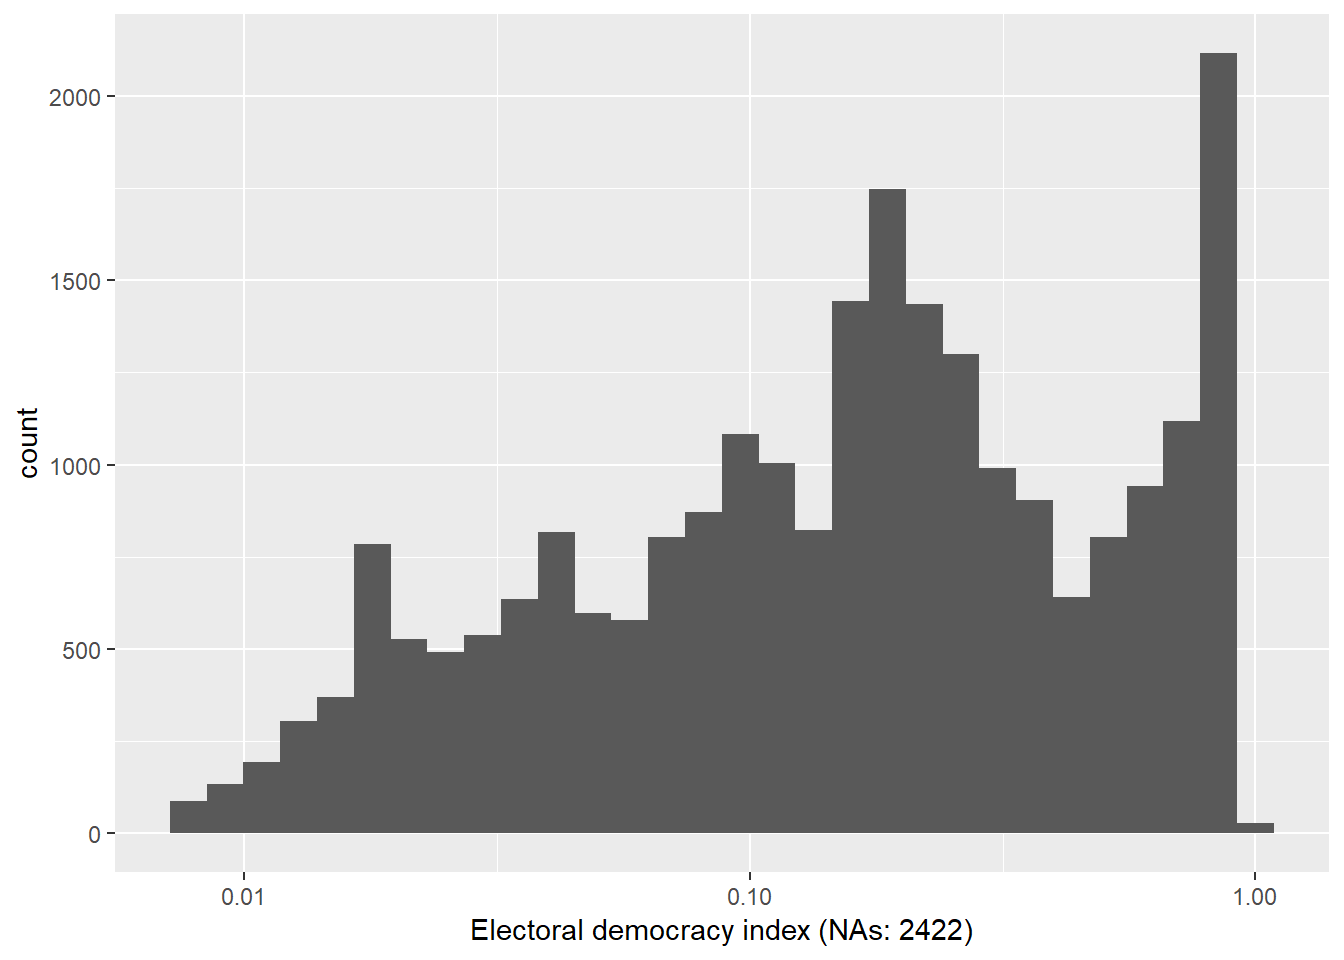
\includegraphics{bachelor-thesis_files/figure-latex/unnamed-chunk-26-1.pdf}

I refer to the documentation for more details.

Another independent layer function is given by \texttt{fxi\_labeller}
which provides the labeller for a facetting variable. Facetting
variables are specified in the argument \texttt{facet\_vars} and need to
be captured by the function \texttt{vars()}:

\begin{Shaded}
\begin{Highlighting}[]
\NormalTok{diamonds }\OperatorTok\StringTok{ }
\StringTok{  }\KeywordTok{filter}\NormalTok{(color }\OperatorTok\StringTok{ }\NormalTok{LETTERS[}\DecValTok{4}\OperatorTok{:}\DecValTok{6}\NormalTok{]) }\OperatorTok\StringTok{ }
\StringTok{  }\KeywordTok{fx_ggplot}\NormalTok{(}\KeywordTok{aes}\NormalTok{(}\DataTypeTok{x =}\NormalTok{ carat, }\DataTypeTok{y =}\NormalTok{ price), }\DataTypeTok{facet_vars =} \KeywordTok{vars}\NormalTok{(color)) }
\end{Highlighting}
\end{Shaded}

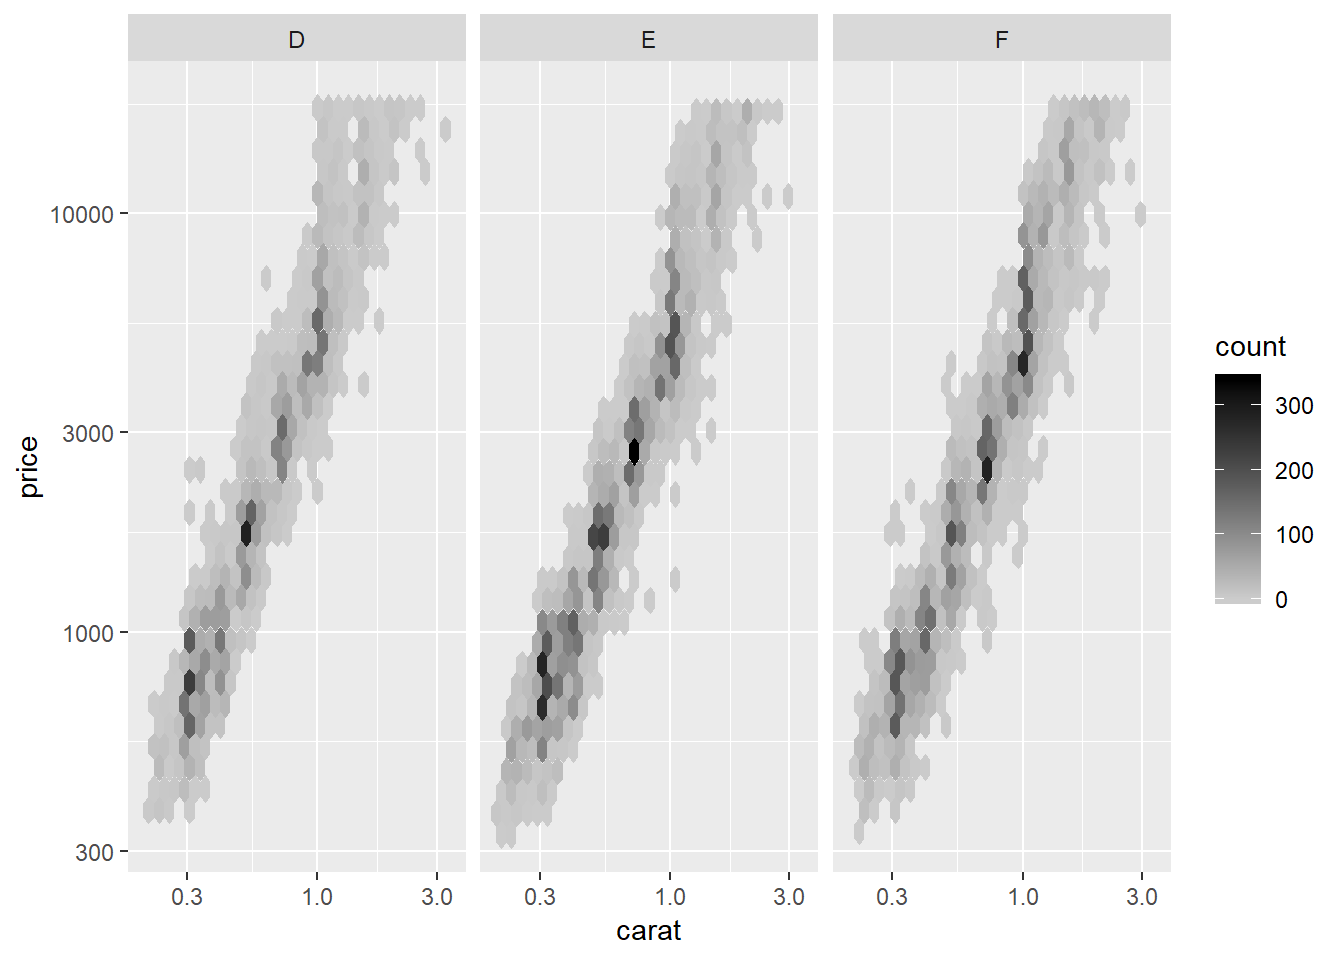
\includegraphics{bachelor-thesis_files/figure-latex/unnamed-chunk-27-1.pdf}

\subsection{Implementation of the voting
system}\label{implementation-of-the-voting-system}

The dependent layers are determined by the internal function
\texttt{fxi\_layer\_complete}. The nominations are handled by
\texttt{fxe\_layer\_complete\_nominate}, which is dispatched over
\texttt{fx\_geom} and \texttt{aes\_name}, as well. The function accepts
the parameter \texttt{fxGeom\_nominations} which may provide additional
nominations. As these are absence, however, only the default nominations
are provided.

These are handled by the S3 class \texttt{nominations} which returns,
depending on the access function, all layers, scales, facets, coordinate
system or other \texttt{ggproto} objects within a certain nomination
(see the documentation). This will become important for votes and vetos.

The nominations by the x aesthetic can be caught by

\begin{Shaded}
\begin{Highlighting}[]
\NormalTok{x_noms <-}\StringTok{ }\KeywordTok{fxe_layer_complete_nominate}\NormalTok{(}\KeywordTok{fxGeom}\NormalTok{(}\StringTok{"Continuous"}\NormalTok{), }\KeywordTok{AesName}\NormalTok{(}\StringTok{"x"}\NormalTok{), diamonds)}
\end{Highlighting}
\end{Shaded}

As such an object is messy to print, I will simply list the four
nominations:

\begin{itemize}
\tightlist
\item
  \texttt{geom\_point()} with an automatically determined transparency
  value \texttt{alpha}
\item
  \texttt{geom\_histogram()}
\item
  \texttt{geom\_density()}
\item
  \texttt{geom\_hex(),\ scale\_fill\_gradient()} with limits which are
  anchored at 0 and a custom palette.
\end{itemize}

Evidently, these layers are suitable for very different plots. If you
consider which layers to nominate, you can simply choose all that make
sense in some combination. Votes and vetos will take care of the rest.

Besides supplying additional nominations via
\texttt{fxGeom\_nominations}, you can extend the function by importing
the S4 generic and defining a new method.

Going on, the function \texttt{fxe\_layer\_complete\_veto} is
responsible for the vetoes. Its structure is

\begin{verbatim}
fxe_layer_complete_veto(nomination, fx_geom, aes_name, data, ...)
\end{verbatim}

and it dispatches over \texttt{fx\_geom} and \texttt{aes\_name}. The
internal function calls the appopriate method for every nomination. The
method simply returns a boolean where \texttt{FALSE} causes no action
and \texttt{TRUE} indicates that the nomination ought to be removed.
Consider, for instance, the call below:

\begin{Shaded}
\begin{Highlighting}[]
\KeywordTok{fxe_layer_complete_veto}\NormalTok{(}\KeywordTok{nomination}\NormalTok{(}\KeywordTok{geom_density}\NormalTok{()), }\KeywordTok{fxGeom}\NormalTok{(}\StringTok{"Continuous"}\NormalTok{), }\KeywordTok{AesName}\NormalTok{(}\StringTok{"y"}\NormalTok{), diamonds)}
\end{Highlighting}
\end{Shaded}

\begin{verbatim}
## [1] TRUE
\end{verbatim}

This aesthetic vetoes a density plot because this would require a
missing y aesthetic. Consequently, only the scatter plot and the
hexagonal heatmap remain as valid options (all other nominations from
the y aesthetic have been vetoed, as well).

Finally, the following function casts the votes:

\begin{verbatim}
fxe_layer_complete_vote(nomination, fx_geom, aes_name, data, ...)
\end{verbatim}

It dispatches over the same arguments and returns, for a given
nomination an integer which represents the votes for a certain
nomination. In this case, we observe:

\begin{Shaded}
\begin{Highlighting}[]
\KeywordTok{fxe_layer_complete_vote}\NormalTok{(}\KeywordTok{nomination}\NormalTok{(}\KeywordTok{geom_point}\NormalTok{()), }\KeywordTok{fxGeom}\NormalTok{(}\StringTok{"Continuous"}\NormalTok{), }\KeywordTok{AesName}\NormalTok{(}\StringTok{"x"}\NormalTok{), diamonds)}
\end{Highlighting}
\end{Shaded}

\begin{verbatim}
## [1] 0
\end{verbatim}

\begin{Shaded}
\begin{Highlighting}[]
\KeywordTok{fxe_layer_complete_vote}\NormalTok{(}\KeywordTok{nomination}\NormalTok{(}\KeywordTok{geom_hex}\NormalTok{()), }\KeywordTok{fxGeom}\NormalTok{(}\StringTok{"Continuous"}\NormalTok{), }\KeywordTok{AesName}\NormalTok{(}\StringTok{"x"}\NormalTok{), diamonds)}
\end{Highlighting}
\end{Shaded}

\begin{verbatim}
## [1] 2
\end{verbatim}

The same applies to the y aesthetic. Why does the heatmap receive more
votes? The reason lies in the large amount of data -- the threshold at
which the heatmap receives the majority of votes can be determined by
the parameter \texttt{fxGeom\_hex.threshold}.

The hexagonal heatmap therefore receives 4 votes whereas its only rival,
the scatter plot, receives 0 votes. From these steps, the above pictured
plot emerges.

\subsection{Discussion and
alternatives}\label{discussion-and-alternatives}

This subsection discusses the implementation of \texttt{fx\_ggplot},
lists advantages and adresses possible disadvantages.

\subsubsection{Easy extendibility}\label{easy-extendibility}

The partition of the \texttt{fx\_ggplot} functionality into these
partial functions allows the user to build a complex visualization by
many very simple steps; he only needs to think about one scale, one
possible resp. impossible visualization at a time. If a visualization
does not correspond to the user's need, it is simple enough to fix it;
she needs not define an entire new class but only modify certain
parameters and, if a the need for a new class arises, its definition is
both shorter and easier. This corresponds to the philosophy of
\texttt{tectr} that it should be easy to integrate into the common
explorative process of a statistician.

\subsubsection{High flexibility}\label{high-flexibility}

This advantage is as much hypothesis as observation. The aforementioned
easily acquired extension will also easily work with different classes
that have not actually been intended to work together -- they may even
have been specified by different persons. In a rule-based process, it is
not possible to achieve this kind of flexibility, as far as I can see
it.

\subsubsection{What about
intransparency?}\label{what-about-intransparency}

A possible argument against the voting system might be the following:

\begin{quote}
It is very intransparent what arguments will result in which plot. All
these different functions occlude what could better be solved by an
independent and a dependent layer function where the independent layer
function is simply a rule-based process. The amount of time such
detailedness would cost is easily exceeded by the follow-up process
regarding an unsuitable visualization in the voting system where the
user needs to consider three different functions and identify a suitable
solution which he then needs to validate by some kind of testing.
Finally, even when he has found a solution, changes in the functions of
another aesthetic might result in an unsuitable plot once again. The
voting system arises from laziness in the wrong domain and required a
higher effort for an equally good result than a rule-based system.
\end{quote}

As applies to most arguments with regards to programs in such early
stages of development, the most reliable answer would be to wait and see
which system works best. However, I would argue for a few heuristics
that are on my side. Firstly, I would argue that the amount of time for
such an adaptation is limited, as the user can basically follow a -step
program: let us assume that the dependent elements x are shown but the
user would like to see the elements y.

\begin{enumerate}
\def\labelenumi{\arabic{enumi}.}
\tightlist
\item
  See if y is nominated. If it is not, nominate y and see if the plot
  changes.
\item
  See if y is vetoed. If it is, reconsider either the veto or your own
  preferences.
\item
  See if x should be vetoed. If it should, implement the veto and see if
  the plot changes.
\item
  See where x and where y gathers its vote. Change the voter attribution
  at the appropriate place.
\end{enumerate}

At any step, it might become useful to define a new class. However, this
class would be quickly implemented because the user could start with few
definitions whereas the rigidity of the rule-based system appears to me
more vulnerable to modifications.

This also applies to the second part of the argument. Of course, changes
might affect certain plots. However, such a change is, in my estimate,
more likely in a rule-based system, as the voting system cuts the
function some slack and allows the user to demonstrate the importance of
a certain nomination.

\subsubsection{What about numbers?}\label{what-about-numbers}

This is, of course, a good starting point for a new criticism. It is
actually a special case of the intransparency argument:

\begin{quote}
Even if these numbers, if applied properly, supported a useful
visualization system, it is too hard to apply them properly. Humans are
not good at handling arbitrary numbers and in a complex system, the
effect of these numbers is completely intransparent.
\end{quote}

I concede that the introduction of the votes is slightly artificial. I
would argue, however, that the proper remedy is not admitting defeat or
employing a rule-based system but rather to make these numbers less
arbitrary by agreeing on certain standards. After a few application,
analysis of the resulting problems might yield a good guideline.
Complementary to such an approach, an automated system might be able to
compensate human inability. The statistician might be suggested
different corresponding plots for certain variable combination and can
then choose the best among those plots. Following a certain heuristic,
the automated system could infer the appropriate voting patterns.

\subsubsection{What about letting it
go?}\label{what-about-letting-it-go}

\begin{quote}
I agree that the voting system seems to more suitable for automatic
visualization than a rule-based process. Regardless, these automatic
visualizations are a fruitless endeavour. The independent elements yield
a good adpatation of the plot but the dependent elements adress a
problem in a very complicated manner that does not arise as much. In
most cases there are only a few different kinds of plots that are
employed and it is easier to define them directly and from case to case
manually. Such a definition would be improved by integrating independent
elements.
\end{quote}

Again, the most reliable response to this is to try both methods out and
compare the results. However, I would like to raise a different point at
this place: the definition of the dependent elements could very well
occur with the aim of building a few kinds of visualizations. This would
rather be a good heuristic from which to start. After building such a
model, whenever the need of a new visualization arises it should become
increasingly simple to adapt the system such that the new combinations
fit together. Therefore, the very situation that has been described in
the counterargument might also serve as a suitable situation for the
implementation of a voting system.

Nevertheless, the answer to this counter-arguments needs not be binary.
We might very well employ dependent elements with voting system in
certain contexts whereas a simpler solution might be suitable in other
applications.

\subsection{Lifecycle and further
development}\label{lifecycle-and-further-development}

As I have repeatedly remarked in the previous paragraphs, I believe
further validation of the current approach to be crucial. Thus, I
believe \texttt{fx\_ggplot} in its current implementation to be
potentially useful but far from stable. In particular, the internal
nomination and investigation of the plot elements are a bit awkward and
I can imagine that these functionalities should be properly nested in
the \texttt{ggproto} system of \texttt{ggplot2}. However, determining
this need and a suitable implementation requires more practical
experience with the voting system.

I will therefore apply the voting system to more databases to determine
its strengths and weaknesses. In particular, I will consider possible
voting pattern standards and a more suitable implementations of the
internals.

Indeed, a first application can be found in the next chapter.

\chapter{Final Words}\label{final-words}

We have finished a nice book.

\bibliography{bachelor-thesis.bib}


\end{document}
